\documentclass[10pt,a4paper]{report}
\usepackage[utf8]{inputenc}
\usepackage[russian]{babel}
\usepackage[OT1]{fontenc}
\usepackage{amsmath}
\usepackage{amsfonts}
\usepackage{amssymb}
\usepackage{graphicx}
\usepackage{listings}

\begin{document}
\begin{titlepage}
\title{Отчет по предмету "Телекомуникации". "Сетевой форум"}
\author{Скрипаль Б.А.}
\end{titlepage}
\maketitle
\chapter{Задание}
Разработать клиент-серверную систему сетевого форума из сервера сетевого форума и пользовательских клиентов.
\section{Основные возможности сервера}
\begin{enumerate}
\item Прослушивание определенного порта
\item Обработка запросов на подключение по этому порту от клиентов
\item Поддержка работы нескольких клиентов через механизм нитей
\item Регистрация подключившегося клиента
\item Выдача клиенту перечня новых сообщений форума
\item Выдача клиенту иерархического представление форума
\item Прием от клиента сообщения в ветку форума
\item Выдача списка текущих активных пользователей форума
\item Обработка запроса на отключения клиента
\item Принудительное отключение клиента
\end{enumerate}
\section{Основные возможности клиента}
\begin{enumerate}
\item Установление соединения с сервером
\item Посылка регистрационных данных клиента
\item Получение и вывод перечня новых сообщений 
\item Получение и вывод иерархии форума
\item Выбор текущей ветки форума
\item Посылка сообщений в текущую ветку форума
\item Разрыв соединения
\item Обработка ситуации отключения клиента сервером
\end{enumerate}
\chapter{Нефункциональные требования}
\section{Требования к реализации}
Соединение начинает сервер, отправляя приглашение к аутентификации. Далее клиент пересылает свой логин и пароль. После этого пользователь может просматривать форум (его иерархию и отдельные сообщения), оставлять сообщения в выбранную ветку форума. После завершения работы клиент должен разорвать соединение.
\section{Требования к надежности}
Длинна принимаемого сервером пакета должна быть ограничена, для избежания падения сервера. Так же мы должны обрабатывать неправильные (неккоректные) запросы от клиента. В случае с udp так же необходимо реализовать контроль корректной доставки пакетов. Это можно реализовать следующим образом:
\begin{itemize}
\item На сервере организуется буфер пакетов, в котором некоторое время хранятся на сервере
\item Каждому пакету присваивается свой id.
\item В каждом пакете создаются два поля: номер пакета и всего пакетов.
\item Если клиент какое то время не получает все необходимые пакеты, он отправляет за прос серверу на повторную отправку пакетов.
\item Если все пакеты доставленны, то клиент отправляет сообщение об успехе.
\end{itemize}
\section{Накладываемые ограничения}
\begin{enumerate}
\item Ограничение на длинну пакета - все пакеты можно условно разделить на две группы:
\begin{enumerate}
\item Пакеты подтверждения доставки пакета - для данной цели используются пакеты фиксированной длины 2 байта (сообщение "ОК"). Данное сообщение отправляется в качестве подтверждения получения нового сообщения
\item Пакеты содержащие команды пользователя и ответы сервера - в данном случае использовались пакеты длинной 256 символов. Данное ограничение было сделано из следующий соображений: самое длинное (теоретически) сообщение - добавление нового сообщения в форум. Ограничение на длинну сообщения - 150. Команда добавления + разделители занимают суммарно 6 байт. Оставшихся 50 байт (теоретически) должно хватить на задание темы поста.
\end{enumerate}
\item Обрыв сессии (некорректное завершение работы клиентом). При некорректном завершении сессии клиентом он останется в состоянии "online", что является минусом данного протокола.
\item В протоколе отсутствуют возможности создание новой учетной записи, а так же создание новых тем форума.
\end{enumerate}
\chapter{Описание протокола работы}
\section{Описание основных команд пользователя}
\begin{itemize}
\item topics - вывод архитектуры форума в следующем виде: выводится название темы, затем отделенные табуляцией имена "постов" в данной теме с их уникальными идентификаторами.
\item show номер поста - просмотр содержание выбранного поста. При этом в аккаунт пользователя заносится информация о том, что данное сообщение было просмотренно и в дальнейшем оно не будет показываться как новое при аутентификации пользователя. Если указать неверный id, то не выводится никакое сообщение.
\item online - вывод списка активных пользователей. Под термином "активный пользователь" понимается пользователь, присутствующий в данный момент на форуме.
\item add Имя темы\&Название поста\&Содержание поста - добавление нового "поста" в выбранную пользователем ветвь форума. Если имя темы указано неверно, то тема не будет добавлена на сетевой форум.
\item exit - завершение сеанса. После ввода данной команды связь между клиентом и сервером обрывается, и пользователь переходит в состояние оффлайн.
\end{itemize}
\section{Формат команд}
Формат команд был выбран таким образом, что бы язык управления был максимально удобен для человека. Команды устроены следующим образом:
\begin{itemize}
\item Каждая команда начинается с ключевого слова (например topics)
\item Если у команды есть параметр, то он отделяется от ключевого слова пробелом (например show 00001)
\item Если у команды несколько параметров, то они отделяются друг от друга знаком \& (например add Telecom\&Test\&test)
\end{itemize}
\section{Диаграмма организации клиент-серверного обмена}
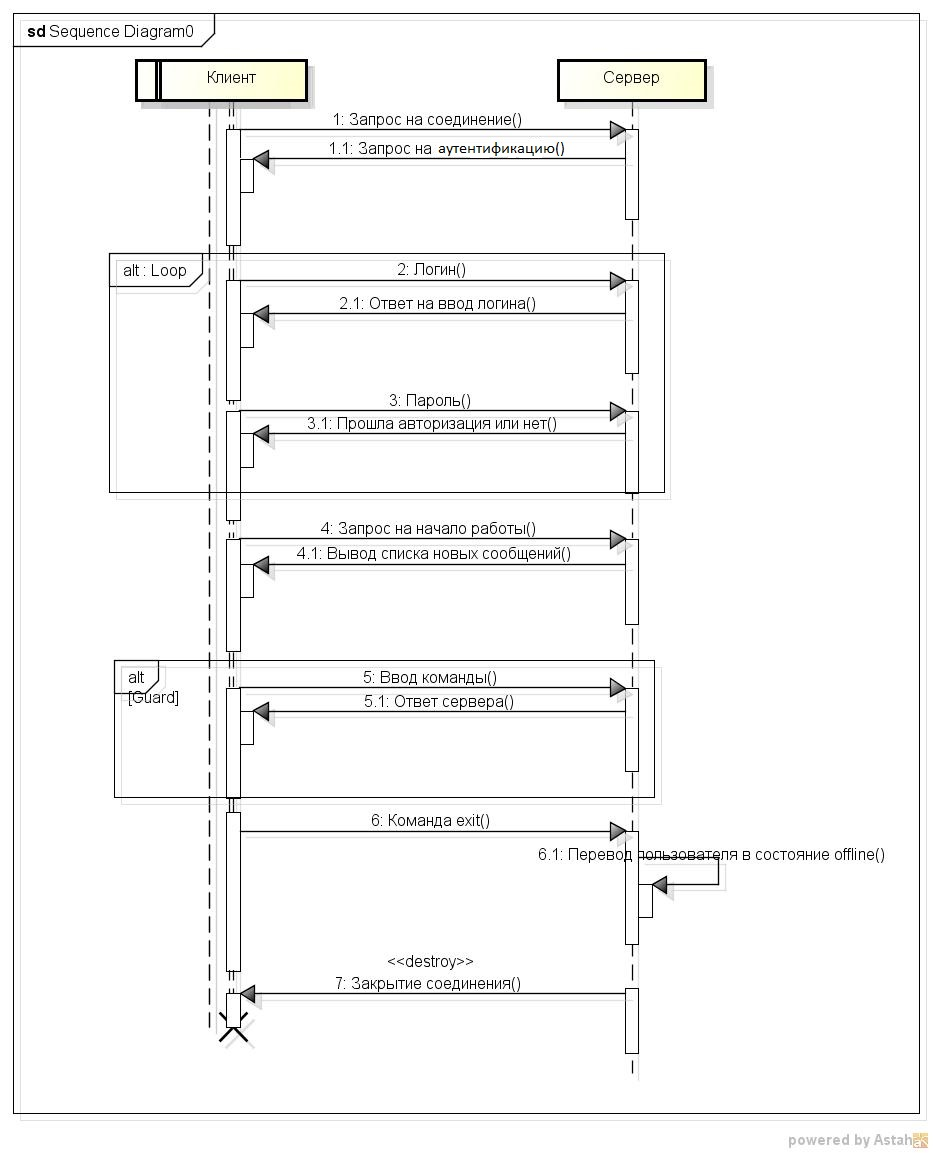
\includegraphics[scale=0.5]{diagram}
\chapter{Архитектура приложения}
\section{Формат хранения данных}
Все данные о пользоветелях, а так же все сообщения форума хранятся в формате XML. К данным о пользователях относится следующее:
\begin{itemize}
\item Уникальный идентификатор пользователя
\item Логин пользователя
\item Пароль пользователя
\item Список просмотренных сообщений
\end{itemize}
Структура форума в представлении XML имеет следующий вид:
\begin{itemize}
\item Каждая тема топика хранится как отдельный тэг. К атрибутам темы относится её имя
\item Внутри каждой темы содержатся список постов форума, относящихся к этой теме. К атрибутам поста отоносится:
\begin{itemize}
\item Уникальный идетнификатор поста
\item Имя поста
\item Содержание сообщения поста
\end{itemize}
\end{itemize}
Для работы с XML-файлами была использована библиотека libxml2. Данная библиотека была выбрана из следующих соображений:
\begin{itemize}
\item Кроссплатформенность - т.к. по заданию было необходимо реализовывать клиентское и серверное приложение под платформы windows и linux, то необходимо что бы используемая библиотека была бы под оба типа операционных систем.
\item Легкость в использовании и большое количество технической документации
\item Надежность
\end{itemize}
В ходе работы приложения используются следующие функции данной библиотеки:
\begin{itemize}
\item Открытие файла для чтения и сохранение изменений в файле
\item Получение потомка
\item Чтение заданных атрибутов потомка, их изменение и сохранение
\end{itemize}
XML-схема структуры файла с содержимым форума
\begin{verbatim}
<xs:schema attributeFormDefault="unqualified" 
elementFormDefault="qualified" xmlns:xs="http://www.w3.org/2001/XMLSchema">
  <xs:element name="topics">
    <xs:complexType>
      <xs:sequence>
        <xs:element name="topic" maxOccurs="unbounded" minOccurs="1">
          <xs:complexType mixed="true">
            <xs:sequence>
              <xs:element name="post" maxOccurs="unbounded" minOccurs="0">
                <xs:complexType>
                  <xs:simpleContent>
                    <xs:extension base="xs:string">
                      <xs:attribute type="xs:byte" name="id"/>
                      <xs:attribute type="xs:string" name="name"/>
                      <xs:attribute type="xs:string" name="autor"/>
                      <xs:attribute type="xs:string" name="text"/>
                    </xs:extension>
                  </xs:simpleContent>
                </xs:complexType>
              </xs:element>
            </xs:sequence>
            <xs:attribute type="xs:string" name="name"/>
          </xs:complexType>
        </xs:element>
      </xs:sequence>
    </xs:complexType>
  </xs:element>
</xs:schema>
\end{verbatim}
XML схема структуры файла с пользователями
\begin{verbatim}
<xs:schema attributeFormDefault="unqualified" 
elementFormDefault="qualified" xmlns:xs="http://www.w3.org/2001/XMLSchema">
  <xs:element name="users">
    <xs:complexType>
      <xs:sequence>
        <xs:element name="user" maxOccurs="unbounded" minOccurs="1">
          <xs:complexType>
            <xs:simpleContent>
              <xs:extension base="xs:string">
                <xs:attribute type="xs:string" name="login"/>
                <xs:attribute type="xs:string" name="password"/>
                <xs:attribute type="xs:byte" name="id"/>
                <xs:attribute type="xs:string" name="view"/>
                <xs:attribute type="xs:string" name="stat"/>
              </xs:extension>
            </xs:simpleContent>
          </xs:complexType>
        </xs:element>
      </xs:sequence>
    </xs:complexType>
  </xs:element>
</xs:schema>
\end{verbatim}
\section{Описание реализации многопоточности}
При подключении нового клиента к серверу ему выделяется отдельный поток. В реализации при помощи TCP все потоки работают параллельно. В UDP пришлось вставить некоторую задержку, для более стабильной работы приложения. Поток закрывается или после отключения клиента от сервера или посредством отключения клиента от сервера посредством сервера. Так как в TCP имеется возможность установления соединения, то каждый поток, фактически, слушает только своего клиента. Из-за того, что в UDP нет такого понятия как соединение, то порт слушается в главном потоке. Затем он определяет какому потоку предназначено это сообщение и записывает его в соответствующую структуру. Потоки, выделенные для клиентов, поочередно просматривают эту структуру и если в ней имеется сообщение для этого потока, то они обрабатывают это сообщение и посылают ответ клиенту.
\section{Анализ уязвимостей приложения}
Для анализа уязвимостей в приложении используем утилиту cppcheck.
Листинг результатов работы утилиты:
\begin{lstlisting}
<?xml version="1.0" encoding="UTF-8"?>
<results version="2">
    <cppcheck version="1.67"/>
    <errors>
        <error id="redundantAssignment" severity="performance"
         msg="Variable &amp;#039;n&amp;#039; is reassigned a
          value before the old one has been used." 
          verbose="Variable &amp;#039;n&amp;#039; is reassigned
           a value before the old one has been used.">
            <location file="tcp_serv_win32\tcp_serv_win32
            \win_tcp_serv.cpp" line="299"/>
            <location file="tcp_serv_win32\tcp_serv_win32
            \win_tcp_serv.cpp" line="302"/>
        </error>
        <error id="redundantAssignment" severity="performance"
         msg="Variable &amp;#039;n&amp;#039; is reassigned a 
         value before the old one has been used." 
         verbose="Variable &amp;#039;n&amp;#039; is reassigned 
         a value before the old one has been used.">
            <location file="tcp_serv_win32\tcp_serv_win32
            \win_tcp_serv.cpp" line="302"/>
            <location file="tcp_serv_win32\tcp_serv_win32
            \win_tcp_serv.cpp" line="303"/>
        </error>
        <error id="redundantAssignment" severity="performance"
         msg="Variable &amp;#039;n&amp;#039; is reassigned a 
         value before the old one has been used." 
         verbose="Variable &amp;#039;n&amp;#039; is reassigned
           a value before the old one has been used.">
            <location file="tcp_serv_win32\tcp_serv_win32
            \win_tcp_serv.cpp" line="303"/>
            <location file="tcp_serv_win32\tcp_serv_win32
            \win_tcp_serv.cpp" line="304"/>
        </error>
        <error id="redundantAssignment" severity="performance"
         msg="Variable &amp;#039;n&amp;#039; is reassigned a
          value before the old one has been used." verbose="Variable
           &amp;#039;n&amp;#039; is reassigned a value before 
           the old one has been used.">
            <location file="tcp_serv_win32\tcp_serv_win32\
            win_tcp_serv.cpp" line="326"/>
            <location file="tcp_serv_win32\tcp_serv_win32\
            win_tcp_serv.cpp" line="332"/>
        </error>
        <error id="redundantAssignment" severity="performance"
         msg="Variable &amp;#039;n&amp;#039; is reassigned a
          value before the old one has been used." verbose="Variable
           &amp;#039;n&amp;#039; is reassigned a value before
            the old one has been used.">
            <location file="tcp_serv_win32\tcp_serv_win32
            \win_tcp_serv.cpp" line="500"/>
            <location file="tcp_serv_win32\tcp_serv_win32
            \win_tcp_serv.cpp" line="501"/>
        </error>
        <error id="variableScope" severity="style" 
        msg="The scope of the variable &amp;#039;root_element&
        amp;#039; can be reduced." verbose="The scope of the 
        variable &amp;#039;root_element&amp;#039; can be reduced.
         Warning: Be careful when fixing this message, especially
          when there are inner loops. Here is an example where 
          cppcheck will write that the scope for &amp;#039;i&amp;
          #039; can be reduced:&#10;void f(int x)&#10;{&#10;    
          int i = 0;&#10;    if (x) {&#10;        // it&amp;#039;s
           safe to move &amp;#039;int i = 0;&amp;#039; here&#10; 
          for (int n = 0; n &amp;lt; 10; ++n) {&#10;
          // it is possible but not safe to 
          move &amp;#039;int i = 0;&amp;#039; here&#10;
           do_something(&amp;amp;i);&#10; }&#10; }&#10;}&#10;When 
           you see this message it is always safe to reduce
            the variable scope 1 level.">
            <location file="tcp_serv_win32\tcp_serv_win32
            \win_tcp_serv.cpp" line="242"/>
        </error>
        <error id="variableScope" severity="style" msg="The scope
         of the variable &amp;#039;id&amp;#039; can be reduced." 
         verbose="The scope of the variable &amp;#039;id&amp;#039; 
         can be reduced. Warning: Be careful when fixing this message, 
         especially when there are inner loops. Here is an example 
         where cppcheck will write that the scope for &amp;#039;i&
         amp;#039; can be reduced:&#10;void f(int x)&#10;{&#10;    
         int i = 0;&#10;    if (x) {&#10;        // it&amp;#039;
         s safe to move &amp;#039;int i = 0;&amp;#039; here&#10;  
         for (int n = 0; n &amp;lt; 10; ++n) {&#10;            
         // it is possible but not safe to move &amp;#039;int i = 0;
         &amp;#039; here&#10;            do_something(&amp;amp;i);&#10;        
         }&#10;    }&#10;}&#10;When you see this message it is always 
         safe to reduce the variable scope 1 level.">
            <location file="tcp_serv_win32\tcp_serv_win32\
            win_tcp_serv.cpp" line="293"/>
        </error>
        <error id="variableScope" severity="style" msg="The scope 
        of the variable &amp;#039;root_element&amp;#039; can 
        be reduced." verbose="The scope of the variable &amp;#039;
        root_element&amp;#039; can be reduced. Warning: Be 
        careful when fixing this message, especially when there 
        are inner loops. Here is an example where cppcheck 
        will write that the scope for &amp;#039;i&amp;#039; can 
        be reduced:&#10;void f(int x)&#10;{&#10;    int i = 0;&#10;    
        if (x) {&#10;        // it&amp;#039;s safe to move &amp;
        #039;int i = 0;&amp;#039; here&#10;        for (int n = 0; n 
        &amp;lt; 10; ++n) {&#10;            // it is possible but 
        not safe to move &amp;#039;int i = 0;&amp;#039; here&#10;            
        do_something(&amp;amp;i);&#10;        }&#10;    }&#10;}&#10;
        When you see this message it is always safe to reduce the 
        variable scope 1 level.">
            <location file="tcp_serv_win32\tcp_serv_win32\
            win_tcp_serv.cpp" line="296"/>
        </error>
        <error id="variableScope" severity="style" msg="The scope 
        of the variable &amp;#039;n&amp;#039; can be reduced." 
        verbose="The scope of the variable &amp;#039;n&amp;#039; 
        can be reduced. Warning: Be careful when fixing this 
        message, especially when there are inner loops. Here is an 
        example where cppcheck will write that the scope for &amp;
        #039;i&amp;#039; can be reduced:&#10;void f(int x)&#10;{&#10;    
        int i = 0;&#10;    if (x) {&#10;        // it&amp;#039;s safe
         to move &amp;#039;int i = 0;&amp;#039; here&#10;        
         for (int n = 0; n &amp;lt; 10; ++n) {&#10;            
         // it is possible but not safe to move &amp;#039;
         int i = 0;&amp;#039; here&#10;            
         do_something(&amp;amp;i);&#10;        }&#10;    
         }&#10;}&#10;When you see this message it is always 
         safe to reduce the variable scope 1 level.">
            <location file="tcp_serv_win32\tcp_serv_win32\
            win_tcp_serv.cpp" line="489"/>
        </error>
        <error id="unreadVariable" severity="style" 
        msg="Variable &amp;#039;j&amp;#039; is assigned 
        a value that is never used." verbose="Variable &
        amp;#039;j&amp;#039; is assigned a value that is never used.">
            <location file="tcp_serv_win32\tcp_serv_win32\
            win_tcp_serv.cpp" line="90"/>
        </error>
        <error id="unreadVariable" severity="style" 
        msg="Variable &amp;#039;n&amp;#039; is assigned 
        a value that is never used." verbose="Variable &amp;
        #039;n&amp;#039; is assigned a value that is never used.">
            <location file="tcp_serv_win32\tcp_serv_win32\
            win_tcp_serv.cpp" line="332"/>
        </error>
        <error id="unreadVariable" severity="style" 
        msg="Variable &amp;#039;n&amp;#039; is assigned a 
        value that is never used." verbose="Variable &amp;
        #039;n&amp;#039; is assigned a value that is never used.">
            <location file="tcp_serv_win32\tcp_serv_win32\
            win_tcp_serv.cpp" line="501"/>
        </error>
        <error id="redundantAssignment" severity="performance" 
        msg="Variable &amp;#039;n&amp;#039; is reassigned a value 
        before the old one has been used." verbose="Variable &amp;
        #039;n&amp;#039; is reassigned a value before the old 
        one has been used.">
            <location file="client_tcp_lin\main.c" line="62"/>
            <location file="client_tcp_lin\main.c" line="68"/>
        </error>
        <error id="redundantAssignment" severity="performance" 
        msg="Variable &amp;#039;n&amp;#039; is reassigned a value 
        before the old one has been used." verbose="Variable &amp;
        #039;n&amp;#039; is reassigned a value before the old one
         has been used.">
            <location file="server_tcp_lin\main.c" line="149"/>
            <location file="server_tcp_lin\main.c" line="152"/>
        </error>
        <error id="redundantAssignment" severity="performance" 
        msg="Variable &amp;#039;n&amp;#039; is reassigned a 
        value before the old one has been used." 
        verbose="Variable &amp;#039;n&amp;#039; is reassigned a 
        value before the old one has been used.">
            <location file="server_tcp_lin\main.c" line="337"/>
            <location file="server_tcp_lin\main.c" line="340"/>
        </error>
        <error id="redundantAssignment" severity="performance" 
        msg="Variable &amp;#039;n&amp;#039; is reassigned a 
        value before the old one has been used." verbose="Variable 
        &amp;#039;n&amp;#039; is reassigned a value before the old
         one has been used.">
            <location file="server_tcp_lin\main.c" line="346"/>
            <location file="server_tcp_lin\main.c" line="347"/>
        </error>
        <error id="variableScope" severity="style" 
        msg="The scope of the variable &amp;#039;root_element&amp;#039; 
        can be reduced." verbose="The scope of the variable &amp;#039;
        root_element&amp;#039; can be reduced. Warning: Be careful 
        when fixing this message, especially when there are inner 
        loops. Here is an example where cppcheck will write that 
        the scope for &amp;#039;i&amp;#039; can be reduced:&#10
        void f(int x)&#10;{&#10;    int i = 0;&#10;    if (x) {&#10;        
        // it&amp;#039;s safe to move &amp;#039;int i = 0;&amp;#039; 
        here&#10;        for (int n = 0; n &amp;lt; 10; ++n) {&#10;            
        // it is possible but not safe to move &amp;#039;int i = 0;
        &amp;#039; here&#10;            do_something(&amp;amp;i);&#10;        
        }&#10;    }&#10;}&#10;When you see this message it is
         always safe to reduce the variable scope 1 level.">
            <location file="server_tcp_lin\main.c" line="269"/>
        </error>
        <error id="variableScope" severity="style" 
        msg="The scope of the variable &amp;#039;id&amp;#039; 
        can be reduced." verbose="The scope of the variable &amp;#039;
        id&amp;#039; can be reduced. Warning: Be careful when 
        fixing this message, especially when there are inner loops. 
        Here is an example where cppcheck will write that the scope 
        for &amp;#039;i&amp;#039; can be reduced:&#10;void f(int x)
        &#10;{&#10;    int i = 0;&#10;    if (x) {&#10;        
        // it&amp;#039;s safe to move &amp;#039;int i = 0;&amp;#039; 
        here&#10;        for (int n = 0; n &amp;lt; 10; ++n) {&#10;           
         // it is possible but not safe to move &amp;#039;int 
         i = 0;&amp;#039; here&#10;            do_something(&amp;amp;i);
         &#10;        }&#10;    }&#10;}&#10;When you see this message
          it is always safe to reduce the variable scope 1 level.">
            <location file="server_tcp_lin\main.c" line="330"/>
        </error>
        <error id="variableScope" severity="style" 
        msg="The scope of the variable &amp;#039;root_element&amp;
        #039; can be reduced." verbose="The scope of the variable &amp;
        #039;root_element&amp;#039; can be reduced. Warning: 
        Be careful when fixing this message, especially when 
        there are inner loops. Here is an example where cppcheck 
         write that the scope for &amp;#039;i&amp;#039; can be reduced:
         &#10;void f(int x)&#10;{&#10;    int i = 0;&#10;    if (x) {&#10;        
         // it&amp;#039;s safe to move &amp;#039;int i = 0;&amp;#039; here&#10;        
         for (int n = 0; n &amp;lt; 10; ++n) {&#10;            
         // it is possible but not safe to move &amp;#039;int i = 0;
         &amp;#039; here&#10;            do_something(&amp;amp;i);&#10;        
         }&#10;    }&#10;}&#10;When you see this message it is always
          safe to reduce the variable scope 1 level.">
            <location file="server_tcp_lin\main.c" line="333"/>
        </error>
        <error id="unusedVariable" severity="style" 
        msg="Unused variable: mainthread" verbose="Unused variable: mainthread">
            <location file="server_tcp_lin\main.c" line="62"/>
        </error>
        <error id="variableScope" severity="style" msg="The scope of 
        the variable &amp;#039;root_element&amp;#039; can be reduced."
         verbose="The scope of the variable &amp;#039;root_element
         &amp;#039; can be reduced. Warning: Be careful when fixing 
         this message, especially when there are inner loops. Here is
          an example where cppcheck will write that the scope for &amp
          ;#039;i&amp;#039; can be reduced:&#10;void f(int x)&#10;{&#10;   
           int i = 0;&#10;    if (x) {&#10;        // it&amp;#039;s safe
            to move &amp;#039;int i = 0;&amp;#039; here&#10;        for 
            (int n = 0; n &amp;lt; 10; ++n) {&#10;            // it is possible 
            but not safe to move &amp;#039;int i = 0;&amp;#039; here&#10;           
             do_something(&amp;amp;i);&#10;        }&#10;    }&#10;}&#10;
             When you see this message it is always safe to reduce the 
             variable scope 1 level.">
            <location file="server_udp_lin\main.c" line="324"/>
        </error>
        <error id="variableScope" severity="style" msg="The scope of the 
        variable &amp;#039;id&amp;#039; can be reduced." verbose="The 
        scope of the variable &amp;#039;id&amp;#039; can be reduced. 
        Warning: Be careful when fixing this message, especially when 
        there are inner loops. Here is an example where cppcheck will 
        write that the scope for &amp;#039;i&amp;#039; can be reduced:
        &#10;void f(int x)&#10;{&#10;    int i = 0;&#10;    if (x) {&#10;        
        // it&amp;#039;s safe to move &amp;#039;int i = 0;&amp;#039; 
        here&#10;        for (int n = 0; n &amp;lt; 10; ++n) {&#10;            
        // it is possible but not safe to move &amp;#039;int i = 0;&amp;
        #039; here&#10;            do_something(&amp;amp;i);&#10;        
        }&#10;    }&#10;}&#10;When you see this message it is always safe 
        to reduce the variable scope 1 level.">
            <location file="server_udp_lin\main.c" line="424"/>
        </error>
        <error id="variableScope" severity="style" msg="The scope 
        of the variable &amp;#039;root_element&amp;#039; can be 
        reduced." verbose="The scope of the variable &amp;#039;
        root_element&amp;#039; can be reduced. Warning: Be careful 
        when fixing this message, especially when there are inner 
        loops. Here is an example where cppcheck will write that 
        the scope for &amp;#039;i&amp;#039; can be reduced:&#10;
        void f(int x)&#10;{&#10;    int i = 0;&#10;    if (x) {&#10;        
        // it&amp;#039;s safe to move &amp;#039;int i = 0;&amp;#039;
         here&#10;        for (int n = 0; n &amp;lt; 10; ++n) {&#10;            
         // it is possible but not safe to move &amp;#039;int i = 0;
         &amp;#039; here&#10;            do_something(&amp;amp;i);&#10;        
         }&#10;    }&#10;}&#10;When you see this message it is 
         always safe to reduce the variable scope 1 level.">
            <location file="server_udp_lin\main.c" line="427"/>
        </error>
        <error id="redundantAssignment" severity="performance" 
        msg="Variable &amp;#039;n&amp;#039; is reassigned a value
         before the old one has been used." verbose="Variable &amp;
         #039;n&amp;#039; is reassigned a value before the old one
          has been used.">
            <location file="server_udp_win32\server_udp_win32
            \server_udp_win32.cpp" line="494"/>
            <location file="server_udp_win32\server_udp_win32
            \server_udp_win32.cpp" line="500"/>
        </error>
        <error id="variableScope" severity="style" msg="The scope 
        of the variable &amp;#039;root_element&amp;#039; can be
         reduced." verbose="The scope of the variable &amp;#039;
         root_element&amp;#039; can be reduced. Warning: Be careful
         when fixing this message, especially when there are inner
          loops. Here is an example where cppcheck will write that
           the scope for &amp;#039;i&amp;#039; can be reduced:&#10;
           void f(int x)&#10;{&#10;    int i = 0;&#10;    if (x) {&#10;
                   // it&amp;#039;s safe to move &amp;#039;int i = 0;
                   &amp;#039; here&#10;        for (int n = 0; n &amp;
                   lt; 10; ++n) {&#10;            // it is possible 
                   but not safe to move &amp;#039;int i = 0;&amp;
                   #039; here&#10;            do_something(&amp;amp;i);&
                   #10;        }&#10;    }&#10;}&#10;When you see this
                    message it is always safe to reduce the variable
                     scope 1 level.">
            <location file="server_udp_win32\server_udp_win32\
            server_udp_win32.cpp" line="383"/>
        </error>
        <error id="variableScope" severity="style" 
        msg="The scope of the variable &amp;#039;id&amp;#039
        ; can be reduced." verbose="The scope of the variable
         &amp;#039;id&amp;#039; can be reduced. Warning: Be
          careful when fixing this message, especially when 
          there are inner loops. Here is an example where 
          cppcheck will write that the scope for &amp;#039;
          i&amp;#039; can be reduced:&#10;void f(int x)&#10;
          {&#10;    int i = 0;&#10;    if (x) {&#10;        
          // it&amp;#039;s safe to move &amp;#039;int i = 0;
          &amp;#039; here&#10;        for (int n = 0; n &amp;lt;
           10; ++n) {&#10;            // it is possible 
           but not safe to move &amp;#039;int i = 0;&amp;
           #039; here&#10;            do_something(&amp;amp;
           i);&#10;        }&#10;    }&#10;}&#10;When you
            see this message it is always safe to reduce the
             variable scope 1 level.">
            <location file="server_udp_win32\server_udp_win32
            \server_udp_win32.cpp" line="446"/>
        </error>
        <error id="variableScope" severity="style" 
        msg="The scope of the variable &amp;#039;root_element
        &amp;#039; can be reduced." verbose="The scope of the
         variable &amp;#039;root_element&amp;#039; can be 
         reduced. Warning: Be careful when fixing this message,
          especially when there are inner loops. Here is an 
          example where cppcheck will write that the scope for
           &amp;#039;i&amp;#039; can be reduced:&#10;void 
           f(int x)&#10;{&#10;    int i = 0;&#10;    if (x) {&#10;        
           // it&amp;#039;s safe to move &amp;#039;int i = 0;&amp;
           #039; here&#10;        for (int n = 0; n &amp;lt; 10; ++n) 
           {&#10;            // it is possible but not safe to move 
           &amp;#039;int i = 0;&amp;#039; here&#10;           
            do_something(&amp;amp;i);&#10;        }&#10;    }&#10;}
            &#10;When you see this message it is always safe to 
            reduce the variable scope 1 level.">
            <location file="server_udp_win32\server_udp_win32
            \server_udp_win32.cpp" line="449"/>
        </error>
        <error id="variableScope" severity="style" msg="The 
        scope of the variable &amp;#039;n&amp;#039; can be 
        reduced." verbose="The scope of the variable &amp;#039
        ;n&amp;#039; can be reduced. Warning: Be careful 
        when fixing this message, especially when there are
         inner loops. Here is an example where cppcheck 
         will write that the scope for &amp;#039;i&amp;#039
         ; can be reduced:&#10;void f(int x)&#10;{&#10;    
         int i = 0;&#10;    if (x) {&#10;        
         // it&amp;#039;s safe to move &amp;#039;int i = 0;
         &amp;#039; here&#10;        for (int n = 0; n &amp;lt;
          10; ++n) {&#10;            // it is possible but not
           safe to move &amp;#039;int i = 0;&amp;#039; here&#10;
            do_something(&amp;amp;i);&#10;        
            }&#10;    }&#10;}&#10;When you see this message
             it is always safe to reduce the variable scope 1 level.">
            <location file="server_udp_win32\server_udp_win32
            \server_udp_win32.cpp" line="690"/>
        </error>
        <error id="unusedStructMember" severity="style" 
        msg="struct or union member &amp;#039;sockParams::
        sockfd&amp;#039; is never used." verbose="struct or
         union member &amp;#039;sockParams::sockfd&amp;#039; is never used.">
            <location file="server_udp_win32\server_udp_win32
            \server_udp_win32.cpp" line="102"/>
        </error>
        <error id="unusedStructMember" severity="style" 
        msg="struct or union member &amp;#039;sockParams:
        :newsockfd&amp;#039; is never used." verbose="struct 
        or union member &amp;#039;sockParams::newsockfd&amp;#039;
         is never used.">
            <location file="server_udp_win32\server_udp_win32
            \server_udp_win32.cpp" line="102"/>
        </error>
        <error id="unusedStructMember" severity="style" 
        msg="struct or union member &amp;#039;sockParams::
        port_number&amp;#039; is never used." verbose="struct 
        or union member &amp;#039;sockParams::port_number&amp
        ;#039; is never used.">
            <location file="server_udp_win32\server_udp_win32
            \server_udp_win32.cpp" line="102"/>
        </error>
        <error id="unusedStructMember" severity="style"
         msg="struct or union member &amp;#039;sockParams::
         client&amp;#039; is never used." verbose="struct or 
         union member &amp;#039;sockParams::client&amp;#039; 
         is never used.">
            <location file="server_udp_win32\server_udp_win32
            \server_udp_win32.cpp" line="102"/>
        </error>
        <error id="unusedStructMember" severity="style" 
        msg="struct or union member &amp;#039;sockParams::countnumber&
        amp;#039; is never used." verbose="struct or union member &amp
        ;#039;sockParams::countnumber&amp;#039; is never used.">
            <location file="server_udp_win32\server_udp_win32
            \server_udp_win32.cpp" line="102"/>
        </error>
        <error id="unreadVariable" severity="style"
         msg="Variable &amp;#039;n&amp;#039; is assigned a value 
         that is never used." verbose="Variable &amp;#039;n&amp;#039;
         is assigned a value that is never used.">
            <location file="server_udp_win32\server_udp_win32
            \server_udp_win32.cpp" line="76"/>
        </error>
        <error id="unusedVariable" severity="style" 
        msg="Unused variable: port" verbose="Unused variable:
         port">
            <location file="server_udp_win32\server_udp_win32\
            server_udp_win32.cpp" line="117"/>
        </error>
        <error id="unusedVariable" severity="style" 
        msg="Unused variable: addr" verbose="Unused variable: addr">
            <location file="server_udp_win32\server_udp_win32
            \server_udp_win32.cpp" line="117"/>
        </error>
        <error id="unreadVariable" severity="style" 
        msg="Variable &amp;#039;thread&amp;#039; is assigned a 
        value that is never used." verbose="Variable &amp;#039;
        thread&amp;#039; is assigned a value that is never used.">
            <location file="server_udp_win32\server_udp_win32
            \server_udp_win32.cpp" line="215"/>
        </error>
        <error id="unreadVariable" severity="style" 
        msg="Variable &amp;#039;slen&amp;#039; is assigned a 
        value that is never used." verbose="Variable &amp;#039;
        slen&amp;#039; is assigned a value that is never used.">
            <location file="server_udp_win32\server_udp_win32\
            server_udp_win32.cpp" line="147"/>
        </error>
        <error id="unreadVariable" severity="style" 
        msg="Variable &amp;#039;n&amp;#039; is assigned a value 
        that is never used." verbose="Variable &amp;#039;n&amp;
        #039; is assigned a value that is never used.">
            <location file="server_udp_win32\server_udp_win32
            \server_udp_win32.cpp" line="192"/>
        </error>
        <error id="unreadVariable" severity="style" 
        msg="Variable &amp;#039;n&amp;#039; is assigned a value 
        that is never used." verbose="Variable &amp;#039;n&amp;
        #039; is assigned a value that is never used.">
            <location file="server_udp_win32\server_udp_win32
            \server_udp_win32.cpp" line="500"/>
        </error>
        <error id="unreadVariable" severity="style" 
        msg="Variable &amp;#039;n&amp;#039; is assigned a 
        value that is never used." verbose="Variable &amp;#039;
        n&amp;#039; is assigned a value that is never used.">
            <location file="server_udp_win32\server_udp_win32
            \server_udp_win32.cpp" line="701"/>
        </error>
        <error id="invalidscanf_libc" severity="portability"
         msg="scanf without field width limits can crash with 
         huge input data on some versions of libc." 
         verbose="scanf without field width limits can crash 
         with huge input data on libc versions older than 2.13-25.
          Add a field width specifier to fix this problem:&#10;   
           %i =&amp;gt; %3i&#10;&#10;Sample program that can crash
           :&#10;&#10;#include &amp;lt;stdio.h&amp;gt;&#10;int main()
           &#10;{&#10;    int a;&#10;    scanf(&amp;quot;%i&amp;quot;
           , &amp;amp;a);&#10;    return 0;&#10;}&#10;&#10;To make i
            crash:&#10;perl -e &amp;#039;print &amp;quot;5&amp;quot;
            x2100000&amp;#039; | ./a.out">
            <location file="server_udp_win32\server_udp_win32\
            server_udp_win32.cpp" line="127"/>
        </error>
    </errors>
</results>
\end{lstlisting}
Как видно из результата критическое ошибки не были найдены. Среди возможных ошибок были замечания о переносимости и о производительности. Часть из них была исправлена.
\section{Дизайн протокола}
\begin{itemize}
\item Клиент отправляет серверу сообщение о начале работы 
\item В ответ сервер разрешает работу клиента. На стороне клиента появляется сообщение "Enter login"
\item Клиент вводит свой логин и нажимает клавишу Enter. Логин отправляется серверу, а на стороне клиента появляется приглашение ввести пароль "Enter password"
\item После ввода пароля, если аутентификация прошла успешно, то клиенту выводятся новые ("не прочитанные им") сообщения форума, и начинается ожидание новой команды клиента. Причиной неудачи при аутентификации могут быть следующие:
\begin{itemize}
\item Неправильная пара логин-пароль. В случае если клиент не может вспомнить пароль или логин и хочет выйти, ему достаточно ввести слово "exit" в поле "логин" и сеанс связи прервется.
\item Данный клиент уже находится в состоянии online на сервере
\end{itemize}
\item При вводе пользователем команды topics ему передается структура сетевого форума, а именно список тем и содержащеися в них посты. Посты отделены от тем знаком табуляции. Так же рядом с каждым сообщением выводится его уникальный идентификатор.
\item Для просмотра содержания выбранного сообщения клиентом вводится команда show, после которой следует номер сообщения, например: "show 00001". В этом случае клиенту выведется содержание данного поста.
\item При вводе команды online клиенту выводится список всех пользователей, которые присутствуют на форуме в данный момент. Каждое имя отделено от другого переносом строки
\item Для добавление нового сообщения используется команда add, после которой следуют имя темы, имя нового сообщения и содержание сообщения. Для отделения каждого из атрибуттов используется знак \&. Например "add Telecom\&Example\&This is test topic". Для того, что бы убедиться в том, что тема добавлена в форум, можно набрать команду topics и увидеть новую тему в списке сообщений.
\item Для завершения сеанса клиенту необходимо ввести команду "exit". После этого сеанс закончится и пользователю будет выведено сообщение о завершении работы.
\end{itemize}
\section{Пример работы с приложением}
\begin{verbatim}
Начало сессии
Hello, print you login and password

Print login

Приглашение на ввод пароля
Print password

Вывод новых сообщений
Hello, telecom!

Hello, telecom again!

Test tcp

Ввод команды topics
topics
Topics:
Telecom
	00001	Why i like telecom
	00001	Why i like telecom
	00002	Hello, telecom!
	00001	Why i like telecom
	00002	Hello, telecom!
	00003	Hello, telecom again!
	00001	Why i like telecom
	00002	Hello, telecom!
	00003	Hello, telecom again!
	36753	Test tcp
Other topic
Ввод команды show
show 00001
Because i must love it

Ввод команды online
online
john

ввод команды add
add Telecom&Test&This is test
Writing
topics
Topics:
Telecom
	00001	Why i like telecom
	00001	Why i like telecom
	00002	Hello, telecom!
	00001	Why i like telecom
	00002	Hello, telecom!
	00003	Hello, telecom again!
	00001	Why i like telecom
	00002	Hello, telecom!
	00003	Hello, telecom again!
	36753	Test tcp
	00001	Why i like telecom
	00002	Hello, telecom!
	00003	Hello, telecom again!
	36753	Test tcp
	36754	Test
Other topic

Ввод команды exit
exit
exit
\end{verbatim}
Так же серверное приложение позволяет организовывать работу нескольких клиентов одновременно. В результате проверки не было выявлено никаких ошибок многопоточности.
\chapter{Организация работы при помощи протокола udp}
При организации работы при помощи протокола udp не было внесено значительных изменений в работу приложения. Однако, т.к. в udp нет такого понятия, как установление сессии, в структуру сервера было внесено следующее изменение: был создан массив структур, каждая из которых содержит в себе:
\begin{itemize}
\item Адрес клиента
\item Номер порта клиента
\item Сокет
\item Номер потока, выделенному клиенту
\item Сообщение для данного потока
\item Флаг нового сообщения
\end{itemize}
Далее серверное приложение работает следующим способом:
\begin{enumerate}
\item Сервер получает входящее сообщение
\item Сверяются уже известные адреса клиентов. Если адрес совпадает с адресом полученного сообщения, то данные записываются в соответствующее поле
\item В противном случае выделяется новых поток
\item Каждый поток опрашивает своб структуру. Если есть новые сообщения, то он обрабатывает их и отправляет клиенту. Затем засыпает на небольшой промежуток времени.
\end{enumerate}
\chapter{Приложения}
\section{Приложение 1. Код сервера tcp}
\begin{verbatim}
#define _CRT_SECURE_NO_DEPRECATE
#include <stdio.h>
#include "parser.h"
#include "tree.h"
#include <stdlib.h>
#include <winsock2.h>
#include <ws2tcpip.h>
#include <string.h>
#include <assert.h>

#pragma comment (lib, "Ws2_32.lib")
#pragma comment (lib, "Mswsock.lib")
#pragma comment (lib, "AdvApi32.lib")
#pragma comment (lib, "libxml2.lib")

#define bzero(b,len) (memset((b), '\0', (len)), (void) 0)  
#define bcopy(b1,b2,len) (memmove((b2), (b1), (len)), (void) 0)

#define	BUFSIZE		512
#define	PORT		5001
#define LOGINSIZE	100
#define	MAXUSERS	5

void print_topic_names(char *buffer,xmlNode * a_node,
	 char* mess,int newsockfd);
void print_topic(char *buffer,int newsockfd);
void login_func(int newsockfd,char *log);
void search_user(xmlNode * a_node, char *login,
	 char *password, char *id);
void search_new_topics(char *name,int newsockfg);
void search_topics_by_name(xmlNode * a_node,
	 char *name, char *buffer);
void fnp_post_by_id(char *buffer,xmlNode * a_node,
	 char *id,int newsockfd);
void fnp_post_name_by_id(xmlNode * a_node, char *id,
	int newsockfd);
void search_all_post(xmlNode * a_node,
	 char all_posts[BUFSIZE-1][6],int *j);
void add_see_topic(xmlNode * a_node, char *login, char *topic_id);
void on_off_user(xmlNode * a_node, char *login,int on_off);
void search_online_user(char *buffer,xmlNode * a_node,int newsockfd);
void add_new_topic(char *buffer,xmlNode * a_node,
	 int newsockfd,char *login);
void add_topic(xmlNode * a_node,char *login,
	 char *topic, char *post, char *text, char *id);
void start_work(int newsockfd);
DWORD WINAPI startThread(LPVOID lpParam);

DWORD dwThreadId[MAXUSERS];
HANDLE thread[MAXUSERS];

struct sockParams
{
	int sockfd, newsockfd, port_number, client,countnumber;
	struct sockaddr_in serv_addr, cli_addr;
};

struct userThread
{
	char login[MAXUSERS][LOGINSIZE];
	int socket[MAXUSERS];
	int count;
};

struct userThread usersthr;

DWORD WINAPI workMainTh(LPVOID lpParam)
{
	char buffer[LOGINSIZE];
	int i;
	while(1)
	{
		fgets(buffer,LOGINSIZE-1,stdin);
		for(i=0;i<MAXUSERS;i++)
		{
			if(strcmp(buffer,usersthr.login[i]))
			{
				ExitThread(dwThreadId[i]);
				closesocket(usersthr.socket[i]);
			}
		}
	}
	return 0;
}

int main( int argc, char *argv[] )
{

	HANDLE mainthread;
	DWORD mtID;
	int i,j;
	struct sockParams sp;
	WSADATA wsaData;
	mainthread=CreateThread(NULL, 0, workMainTh, NULL, 0, &mtID);
	WSAStartup(MAKEWORD(2,2),&wsaData);
	usersthr.count=0;
	i=0;
	j=0;
    sp.sockfd = socket(AF_INET, SOCK_STREAM, IPPROTO_TCP);
    bzero((char *) &sp.serv_addr, sizeof(sp.serv_addr));
    sp.port_number = PORT;
    sp.serv_addr.sin_family = AF_INET;
    sp.serv_addr.sin_addr.s_addr = INADDR_ANY;
    sp.serv_addr.sin_port = htons(sp.port_number);
	bind(sp.sockfd, (struct sockaddr *) &sp.serv_addr,
		 sizeof(sp.serv_addr));
    while(1)
    {
    	listen(sp.sockfd,5);
    	sp.client = sizeof(sp.cli_addr);
		sp.newsockfd = accept(sp.sockfd,
			 (struct sockaddr *)&sp.cli_addr, &sp.client);
		sp.port_number=i;
		thread[i] = CreateThread(NULL, 0, startThread,
			 (LPVOID)&sp, 0, &dwThreadId[i]);
		i++;
	}
}

DWORD WINAPI startThread(LPVOID lpParam)
{
	struct sockParams *sp = (struct sockParams *)lpParam;
	start_work(sp->newsockfd);
	return 0;
}

void start_work(int newsockfd)
{
	int  n;
	xmlDoc         *doc = NULL;
	xmlNode        *root_element = NULL;
	const char     *TopicFilename = "topics.xml";
	const char     *UserFilename = "users.xml";
	char buffer[BUFSIZE],
		message[BUFSIZE];
	char id[6];
	char login[LOGINSIZE];

	bzero(login,LOGINSIZE);
	login_func(newsockfd,login);
	strcpy(usersthr.login[usersthr.count],login);
	usersthr.socket[usersthr.count]=newsockfd;
	usersthr.count++;
	bzero(buffer,BUFSIZE);
	strcpy(buffer,"next\n");
	n=send(newsockfd,buffer,7,0);
	while(1)
	{
		bzero(buffer,BUFSIZE);
		bzero(message,BUFSIZE);
		n= recv( newsockfd,buffer,BUFSIZE-1,0);
		printf("Buffer :%s\n",buffer);
			if(!strncmp(buffer,"topics",strlen("topics")))
	    	{
	    		print_topic(message,newsockfd);
	    	}
	    	if(!strncmp(buffer,"online",strlen("online")))
	    	{
	    		doc = xmlReadFile(UserFilename, NULL, 0);
	    	    if (doc == NULL)
	    	    {
	    			printf("error: could not parse file %s\n", UserFilename);
	    	        strcpy(message,"error");
				}
	    	    else
	    		{
	    			root_element = xmlDocGetRootElement(doc);
	    	        search_online_user(message,root_element,newsockfd);
	    	        xmlFreeDoc(doc);
	    	    }
	    		xmlCleanupParser();
	    	}
	    	if(!strncmp(buffer,"show",strlen("show")))
	    	{
	    	    bzero(id,6);
	    	    for(n=5;n<10;n++)
	    			id[n-5]=buffer[n];
	    	        doc = xmlReadFile(TopicFilename, NULL, 0);
	    	        if (doc == NULL)
	    	        {
	    	            printf("error: could not parse file %s\n", TopicFilename);
	    	        }
	    	        else
	    	        {
	    	            root_element = xmlDocGetRootElement(doc);
	    	            fnp_post_by_id(message,root_element,id,newsockfd);
	    	            xmlFreeDoc(doc);
	    	        }
	    	        xmlCleanupParser();
	    	        doc = xmlReadFile(UserFilename, NULL, 0);
	    	        if (doc == NULL)
	    	        {
	    				printf("error: could not parse file %s\n", UserFilename);
	    	            strcpy(message,"Error\n");
	    	        }
	    	        else
	    	        {
	    	            root_element = xmlDocGetRootElement(doc);
	    	            add_see_topic(root_element,login,id);
	    	            xmlSaveFile(UserFilename,doc);
	    	            xmlFreeDoc(doc);
	    	        }
	    	        xmlCleanupParser();
	    	   }
	    	   if(!strncmp(buffer,"exit",strlen("exit")))
	    	   {
	    	        bzero(buffer,BUFSIZE);
	    	        strncpy(message,"exit\n",strlen("exit\n"));
	    	        doc = xmlReadFile(UserFilename, NULL, 0);
	    	        if (doc == NULL)
	    	        {
	    	            printf("error: could not parse file %s\n", UserFilename);
	    	        }
	    	        else
	    	        {
	    	            root_element = xmlDocGetRootElement(doc);
	    	            on_off_user(root_element,login,0);
	    	            xmlSaveFile(UserFilename,doc);
	    	            xmlFreeDoc(doc);
	    	        }
	    	        xmlCleanupParser();
	    	        return;
	    	   }
	    	   if(!strncmp(buffer,"add",3))
	    	   {
	    	        doc = xmlReadFile(TopicFilename, NULL, 0);
	    	        if (doc == NULL)
	    	        {
	    	            printf("error: could not parse file %s\n", TopicFilename);
	    	            strcpy(message,"Error\n");
	    	        }
	    	        else
	    	        {
	    	            root_element = xmlDocGetRootElement(doc);
	    	            add_new_topic(buffer,root_element,newsockfd,login);
	    	            xmlSaveFile(TopicFilename,doc);
	    	            xmlFreeDoc(doc);
	    	        }
	    	        xmlCleanupParser();
	    	    }
	    	    if(message[0]==0)
	    	    {
	    	        strcpy(message,"next");
	    	    }
	    	    n=send(newsockfd,message,strlen(message),0);
	    }
}

void print_topic(char *buffer,int newsockfd)
{

    xmlDoc         *doc = NULL;
    xmlNode        *root_element = NULL;
    const char     *Filename = "topics.xml";
    doc = xmlReadFile(Filename, NULL, 0);
    if (doc == NULL)
    {
        printf("error: could not parse file %s\n", Filename);
    }
    else
    {
        root_element = xmlDocGetRootElement(doc);
         strcpy(buffer,"Topics:\n");
        print_topic_names(buffer,root_element,buffer,newsockfd);
        xmlFreeDoc(doc);
    }
    xmlCleanupParser();
    return;
}

void print_topic_names(char *buffer,xmlNode * a_node, char *mess, int newsockfd)
{
    xmlNode *cur_node = NULL;
    char buf[BUFSIZE];
    bzero(buf,BUFSIZE);
    for (cur_node = a_node; cur_node; cur_node = cur_node->next) {
        if (cur_node->type == XML_ELEMENT_NODE) {
            if((!xmlStrcmp(cur_node->name,(const xmlChar *)"topic")))
            {
                strncpy(buf,(char *)xmlGetProp(cur_node,
                (const xmlChar *)"name"),strlen((char *)xmlGetProp(cur_node,
                (const xmlChar *)"name")));
				
                strcat(buf,"\n");
                strcat(buffer,buf);
            }
            if((!xmlStrcmp(cur_node->name,(const xmlChar *)"post")))
            {
                strcat(buf,"	");
                strncat(buf,(char *)xmlGetProp(cur_node,(const xmlChar *)"id"),
                strlen((char *)xmlGetProp(cur_node,(const xmlChar *)"id")));
                strcat(buf,"	");
                strncat(buf,(char *)xmlGetProp(cur_node,(const xmlChar *)"name"),
                strlen((char *)xmlGetProp(cur_node,(const xmlChar *)"name")));
                strcat(buf,"\n");
                strcat(buffer,buf);
            }
        }
        print_topic_names(buffer,cur_node->children,mess,newsockfd);
    }
}

void login_func(int newsockfd,char * log)
{
	char login[BUFSIZE];
	char password[BUFSIZE];
	int n;
	char id[BUFSIZE];

	xmlDoc         *doc = NULL;
	xmlNode        *root_element = NULL;
	const char     *Filename = "users.xml";
	doc = xmlReadFile(Filename, NULL, 0);
	n = send(newsockfd,"Hello, print you login and password\n",36,0);
	bzero(login,BUFSIZE);
	bzero(password,BUFSIZE);
	n = recv( newsockfd,login,BUFSIZE-1,0);
	n=send(newsockfd,"OK",strlen("OK"),0);
	n = recv( newsockfd,password,BUFSIZE-1,0);
	if (doc == NULL)
	{
		printf("error: could not parse file %s\n", Filename);
	}
	else
	{
		if(!strncmp(login,"exit",strlen("exit")))
			exit(1);
		root_element = xmlDocGetRootElement(doc);
		bzero(id,BUFSIZE);
		login[strlen(login)-1] = 0;
		password[strlen(password)-1] = 0;
	    search_user(root_element,login,password,id);
	    if(id[0] == 0)
	    {
	    	printf("Invalid login --%s-- and password --%s-- \n
	    	 Retry write you login and password\n");
	    	n=send(newsockfd,"OK",strlen("OK"),0);
	    	login_func(newsockfd,login);
	    }
	    else
	    {
	    	n=send(newsockfd,"next",strlen("next"),0);
	    	search_new_topics(login,newsockfd);
	    	root_element = xmlDocGetRootElement(doc);
	    	on_off_user(root_element,login,1);
	    	xmlSaveFile(Filename,doc);
	    	strcpy(log,login);
	    	n=send(newsockfd,"next",strlen("next"),0);
	    }

	    xmlFreeDoc(doc);
	}
	xmlCleanupParser();
	return;
}

void search_user(xmlNode * a_node, char *login, char *password,char *id)
{
	xmlNode *cur_node = NULL;
	for (cur_node = a_node; cur_node; cur_node = cur_node->next) {
		if (cur_node->type == XML_ELEMENT_NODE) {
			if((!xmlStrcmp(cur_node->name,(const xmlChar *)"user")))
			{
				if((!xmlStrcmp(xmlGetProp(cur_node,(const xmlChar *)"login"),
				(const xmlChar *)login)))
				{
					if((!xmlStrcmp(xmlGetProp(cur_node,(const xmlChar *)"password"),
					(const xmlChar *)password)))
						if((!xmlStrcmp(xmlGetProp(cur_node,(const xmlChar *)"stat"),
						(const xmlChar *)"ff")))
						{
							strcpy(id,(char *)xmlGetProp(cur_node,(const xmlChar *)"id"));
							return;
						}
				}
			}
	    }
	        search_user(cur_node->children,login,password,id);
	}
}

void search_new_topics(char *name, int newsockfg)
{
	char all_topics[BUFSIZE][6];
	char user_topics[BUFSIZE][6];
	char new_topics[BUFSIZE][6];
	char buffer[BUFSIZE];
	int i,j,k,i2,j2,k2,ch;
	xmlDoc         *doc = NULL;
	xmlNode        *root_element = NULL;
	const char     *Filename = "users.xml";
	const char	   *Filename2 = "topics.xml";
	doc = xmlReadFile(Filename, NULL, 0);
	for(i = 0; i< BUFSIZE;i++)
	{
		bzero(all_topics[i],6);
		bzero(user_topics[i],6);
		bzero(new_topics[i],6);
	}
	bzero(buffer,BUFSIZE);
	root_element = xmlDocGetRootElement(doc);
	search_topics_by_name(root_element,name,buffer);
	i=0;
	k=0;
	for(i =0; ((k < BUFSIZE-6) && (k<((int)strlen(buffer)-1)));i++)
	{
		for(j=0;j<5;j++)
		{
			user_topics[i][j]=buffer[k];
			k++;
		}
		k++;
	}
	bzero(buffer,BUFSIZE);
	doc = xmlReadFile(Filename2, NULL, 0);
	root_element = xmlDocGetRootElement(doc);
	i2=0;
	search_all_post(root_element,all_topics,&i2);
	xmlFreeDoc(doc);
	ch=0;
	j=0;
	for(k=0;k<i2;k++)
	{
		for(k2=0;k2<i;k2++)
		{
			if(!strncmp(user_topics[k2],all_topics[k],5))
			{
				ch=1;
			}

		}
		if(ch==0)
		{
			strncpy(new_topics[j],all_topics[k],5);
			j++;
		}
		ch =0;
	}
	doc = xmlReadFile(Filename2, NULL, 0);
	root_element = xmlDocGetRootElement(doc);
	for(j2=0;j2<j;j2++)
	{
		fnp_post_name_by_id(root_element,new_topics[j2],newsockfg);
	}
	xmlFreeDoc(doc);
	xmlCleanupParser();
}

void search_topics_by_name(xmlNode * a_node, char *name, char *buffer)
{
	xmlNode *cur_node = NULL;

	for (cur_node = a_node; cur_node; cur_node = cur_node->next) {
		if (cur_node->type == XML_ELEMENT_NODE) {
			if((!xmlStrcmp(cur_node->name,(const xmlChar *)"user")))
			{
				if((!xmlStrcmp(xmlGetProp(cur_node,(const xmlChar *)"login"),
				(const xmlChar *)name)))
				{
					strcpy(buffer,(char *)xmlGetProp(cur_node,(const xmlChar *)"view"));
					return;
				}
			}
	    }
	        search_topics_by_name(cur_node->children,name,buffer);
	}
}

void fnp_post_by_id(char *buffer,xmlNode * a_node, char *id,int newsockfd)
{
    xmlNode *cur_node = NULL;
    char buf[BUFSIZE];
    bzero(buf,BUFSIZE);
    for (cur_node = a_node; cur_node; cur_node = cur_node->next) {
        if (cur_node->type == XML_ELEMENT_NODE) {
            if((!xmlStrcmp(cur_node->name,(const xmlChar *)"post")))
            {
                if((!xmlStrcmp(xmlGetProp(cur_node,(const xmlChar *)"id"),
                (const xmlChar *)id)))
                {
                    strncpy(buf,(char *)xmlGetProp(cur_node,
                    (const xmlChar *)"text"),strlen((char *)xmlGetProp(cur_node,
                    (const xmlChar *)"text")));
                    strcat(buf,"\n");
                    strcpy(buffer,buf);
                    return;
                }
            }
        }
        fnp_post_by_id(buffer,cur_node->children,id,newsockfd);
    }
}

void search_all_post(xmlNode * a_node, char all_posts[BUFSIZE-1][6],int *j)
{
	xmlNode *cur_node = NULL;
	    for (cur_node = a_node; cur_node; cur_node = cur_node->next) {
	        if (cur_node->type == XML_ELEMENT_NODE) {
	            if((!xmlStrcmp(cur_node->name,(const xmlChar *)"post")))
	            {
	            	strncpy(all_posts[*j], (char*)xmlGetProp(cur_node,
	            	(const xmlChar *)"id"),5);
	            	(*j)++;
				}
	        }
	        search_all_post(cur_node->children,all_posts,j);
	    }
}

void fnp_post_name_by_id(xmlNode * a_node, char *id,int newsockfd)
{
	xmlNode *cur_node = NULL;
	int n;
	char buf[BUFSIZE];
	bzero(buf,BUFSIZE);
			for (cur_node = a_node; cur_node; cur_node = cur_node->next) {
				if (cur_node->type == XML_ELEMENT_NODE) {
					if((!xmlStrcmp(cur_node->name,(const xmlChar *)"post")))
					{
						if((!xmlStrcmp(xmlGetProp(cur_node,(const xmlChar *)"id"),
						(const xmlChar *)id)))
						{
							strncpy(buf,(char *)xmlGetProp(cur_node,
							(const xmlChar *)"name"),strlen((char *)xmlGetProp(cur_node,
							(const xmlChar *)"name")));
							strcat(buf,"\n");
							n = send(newsockfd,buf,strlen(buf),0);
							n=recv(newsockfd,buf,BUFSIZE-1,0);
							return;
						}
					}
			    }
				fnp_post_name_by_id(cur_node->children,id,newsockfd);
			}
}

void add_see_topic(xmlNode * a_node, char *login, char *topic_id)
{
	xmlNode *cur_node = NULL;
	char buf[BUFSIZE];
	bzero(buf,BUFSIZE);
	for (cur_node = a_node; cur_node; cur_node = cur_node->next) {
		if (cur_node->type == XML_ELEMENT_NODE) {
			if((!xmlStrcmp(cur_node->name,(const xmlChar *)"user")))
			{
				if((!xmlStrcmp(xmlGetProp(cur_node,(const xmlChar *)"login"),
				(const xmlChar *)login)))
				{
					strncpy(buf,(char *)xmlGetProp(cur_node,(const xmlChar *)"view"),
					strlen((char *)xmlGetProp(cur_node,(const xmlChar *)"view")));
					strncat(buf,topic_id,5);
					strncat(buf," ",1);
					xmlSetProp(cur_node,(const xmlChar *)"view",(const xmlChar *)buf);
					return;
				}
			}
	    }
		printf("%s\n",buf);
		add_see_topic(cur_node->children,login,topic_id);
	}
}
void on_off_user(xmlNode * a_node, char *login,int on_off)
{
	xmlNode *cur_node = NULL;
		char buf[BUFSIZE];
		bzero(buf,BUFSIZE);
		for (cur_node = a_node; cur_node; cur_node = cur_node->next)
		{
			if (cur_node->type == XML_ELEMENT_NODE) {
				if((!xmlStrcmp(cur_node->name,(const xmlChar *)"user")))
				{
					if((!xmlStrcmp(xmlGetProp(cur_node,(const xmlChar *)"login"),
					(const xmlChar *)login)))
					{
						if(on_off==1)
							xmlSetProp(cur_node,(const xmlChar *)"stat",
							(const xmlChar *)"on");
						else
						{
							xmlSetProp(cur_node,(const xmlChar *)"stat",
							(const xmlChar *)"ff");
						}
						return;
					}
				}
		    }
			on_off_user(cur_node->children,login,on_off);
		}
}
void search_online_user(char *buffer,xmlNode * a_node,int newsockfd)
{
    xmlNode *cur_node = NULL;
    for (cur_node = a_node; cur_node; cur_node = cur_node->next)
    {
        if (cur_node->type == XML_ELEMENT_NODE) {
            if((!xmlStrcmp(cur_node->name,(const xmlChar *)"user")))
            {
                if((!xmlStrcmp((const xmlChar *)xmlGetProp(cur_node,
                (const xmlChar *)"stat"),(const xmlChar *)"on")))
                {
                	strcat(buffer,(char *)xmlGetProp(cur_node,
                	(const xmlChar *)"login"));
                }
            }
        }
        search_online_user(buffer,cur_node->children,newsockfd);
    }
}
void add_new_topic(char *buffer,xmlNode * a_node,int newsockfd,char *login)
{
    int n=0,i;
    char topic_name[BUFSIZE];
    char post_name[BUFSIZE];
    char post_message[BUFSIZE];
    char id[6];
    bzero(topic_name,BUFSIZE);
    for(i=4;buffer[i]!='&';i++)
    {
    	topic_name[n]=buffer[i];
    	n++;
    }
    i++;
    bzero(post_name,BUFSIZE);
    n=0;
    for(;buffer[i]!='&';i++)
    {
        post_name[n]=buffer[i];
        n++;
    }
    i++;
    bzero(post_message,BUFSIZE);
    n=0;
        for(;buffer[i]!=0;i++)
        {
            post_message[n]=buffer[i];
            n++;
        }
    post_message[strlen(post_message)-1]=0;
    printf("---%s---%s---%s---\n",topic_name,post_name,post_message);
    bzero(id,6);
    for(i=0;i<5;i++)
        id[i]=(rand()%10+'0');
    add_topic(a_node,login,topic_name,post_name,post_message,id);
}

void add_topic(xmlNode * a_node,char *login, char *topic, char *post,
 char *text, char *id)
{
	xmlNode *cur_node = NULL;
	char buf[BUFSIZE];
	bzero(buf,BUFSIZE);
	for (cur_node = a_node; cur_node; cur_node = cur_node->next)
	{
		if (cur_node->type == XML_ELEMENT_NODE)
		{
			if(!xmlStrcmp(cur_node->name,(const xmlChar *)"topic"))
				if(!xmlStrcmp((const xmlChar *)xmlGetProp(cur_node,
				(const xmlChar *)"name"),(const xmlChar *)topic))
				{
					xmlNodePtr nNode = xmlNewNode(0,(const xmlChar *)"post");
					xmlSetProp(nNode,(const xmlChar *)"id",(const xmlChar *)id);
					xmlSetProp(nNode,(const xmlChar *)"name",(const xmlChar *)post);
					xmlSetProp(nNode,(const xmlChar *)"autor",(const xmlChar *)login);
					xmlSetProp(nNode,(const xmlChar *)"text",(const xmlChar *)text);
					xmlAddChild(cur_node,nNode);
					return;
				}
		}
		add_topic(cur_node->children,login, topic, post, text, id);
	}
}

\end{verbatim}
\section{Приложение 2. Код клиента tcp}
\begin{verbatim}
#include <stdio.h>
#include <stdlib.h>
#include <winsock2.h>
#include <ws2tcpip.h>
#include <string.h>
#include <assert.h>

#pragma comment (lib, "Ws2_32.lib")
#pragma comment (lib, "Mswsock.lib")
#pragma comment (lib, "AdvApi32.lib")

#define bzero(b,len) (memset((b), '\0', (len)), (void) 0)  
#define bcopy(b1,b2,len) (memmove((b2), (b1), (len)), (void) 0)

#define BUFSIZE 512
#define SERVER	"127.0.0.1"
#define	PORT	5001

int main(int argc, char *argv[])
{
	SOCKET sockfd;
    struct sockaddr_in serv_addr;
    struct hostent *server;
    char buffer[BUFSIZE],
		message[BUFSIZE];
	WSADATA wsaData;

	WSAStartup(MAKEWORD(2,2),&wsaData);
	sockfd = socket(AF_INET, SOCK_STREAM, IPPROTO_TCP);
    if (sockfd == INVALID_SOCKET)
    {
        perror("ERROR opening socket");
        exit(1);
    }
	server = gethostbyname(SERVER);
	if (server == NULL) {
		fprintf(stderr,"ERROR, no such host\n");
		exit(0);
	}
	bzero((char *) &serv_addr, sizeof(serv_addr));
	serv_addr.sin_family = AF_INET;
	bcopy((char *)server->h_addr,
	(char *)&serv_addr.sin_addr.s_addr,
	server->h_length);
	serv_addr.sin_port = htons(PORT);
    if (connect(sockfd,(sockaddr *)&serv_addr,sizeof(serv_addr)) > 0)
    {
         perror("ERROR connecting");
         exit(1);
    }
	while(1)
	{
		bzero(buffer,BUFSIZE);
		recv(sockfd,buffer,BUFSIZE-1,0);	
		printf("%s\n",buffer);
		bzero(message,BUFSIZE);
		printf("Print login\n");
		fgets(message,BUFSIZE-1,stdin);
		send(sockfd,message,strlen(message),0);
		bzero(buffer,BUFSIZE);
		recv(sockfd,buffer,BUFSIZE-1,0);
		bzero(message,BUFSIZE);
		printf("Print password\n");
		fgets(message,BUFSIZE-1,stdin);
		send(sockfd,message,strlen(message),0);
		bzero(buffer,BUFSIZE);
		recv(sockfd,buffer,BUFSIZE-1,0);
		if((!strncmp(buffer,"next",4)))
		{
    		bzero(message,BUFSIZE);
    		strncpy_s(message,"OK",2);
			send(sockfd,buffer,strlen(buffer),0);
    		break;
		}
	}
    while(1)
    {
    	bzero(buffer,BUFSIZE);
		recv(sockfd,buffer,BUFSIZE-1,0);
    	if(strncmp(buffer,"OK",strlen("OK")))
    	{
    		if(strncmp(buffer,"next",strlen("next")))
    			printf("%s\n",buffer);
    	}

    	if(!(strncmp(buffer,"next",strlen("next"))))
    	{
    		printf("Writing\n");
    		bzero(message,BUFSIZE);
    		fgets(message,BUFSIZE-1,stdin);
			send(sockfd,message,strlen(message),0);
			recv(sockfd,buffer,BUFSIZE-1,0);
			send(sockfd,"next",strlen("next"),0);
    	}
    	else
    	{
    		bzero(message,BUFSIZE);
    		strncpy_s(message,"OK",strlen("OK"));
			send(sockfd,message,strlen(message),0);
    	}
    }
}
\end{verbatim}
\section{Приложение 3. Код сервера udp}
\begin{verbatim}
#define _CRT_SECURE_NO_DEPRECATE
#include <stdio.h>
#include <stdlib.h>
#include <winsock2.h>
#include <ws2tcpip.h>
#include <string.h>
#include <assert.h>
#include <libxml/parser.h>
#include <libxml/tree.h>

#pragma comment (lib, "Ws2_32.lib")
#pragma comment (lib, "Mswsock.lib")
#pragma comment (lib, "AdvApi32.lib")
#pragma comment (lib, "libxml2.lib")

#define bzero(b,len) (memset((b), '\0', (len)), (void) 0)  
#define bcopy(b1,b2,len) (memmove((b2), (b1), (len)), (void) 0)

void print_topic_names(char*buffer,xmlNode * a_node, char* mess,int newsockfd);
void print_topic(char *buffer,int newsockfd);
void login_func(int newsockfd,char *log);
void search_user(xmlNode * a_node, char *login, char *password, char *id);
void search_new_topics(char *name,int newsockfg);
void search_topics_by_name(xmlNode * a_node, char *name, char *buffer);
void fnp_post_by_id(char *buffer,xmlNode * a_node, char *id,int newsockfd);
void fnp_post_name_by_id(xmlNode * a_node, char *id,int newsockfd);
void search_all_post(xmlNode * a_node, char all_posts[255][6],int *j);
void add_see_topic(xmlNode * a_node, char *login, char *topic_id);
void on_off_user(xmlNode * a_node, char *login,int on_off);
void search_online_user(char *buffer,xmlNode * a_node,int newsockfd);
void add_new_topic(char *buffer,xmlNode * a_node,int newsockfd,char *login);
void add_topic(xmlNode * a_node,char *login, char *topic, char *post, char *text, char *id);
void start_work(int newsockfd);
DWORD WINAPI startThread(LPVOID lpParam);

#define PORT 8888
#define BUFLEN 512

DWORD dwThreadId[5];

struct connection {
    int recv;
    char data[255];
    struct sockaddr_in addr;
    int socket, addrlen;
};

struct connection conns[20];
int conn_num = 0;

void my_read(int conn, char* data, int length) {
    while (!conns[conn].recv) Sleep(1);
    bcopy(conns[conn].data, data, length);
    conns[conn].recv = 0;
}

int my_write(int conn, char* data, int length) {
    int n;
	printf("%d\n", conns[conn].socket);
	n=sendto(conns[conn].socket, data, length, 0,
		(struct sockaddr*) &conns[conn].addr, conns[conn].addrlen);
	if(n==SOCKET_ERROR)
		printf("Error\n");
	printf("%d \n",n);
	return n;
}

void fill(void* sock) {
    int socketfd = (int) sock;
    int n, i, num;
    char buff[256];
    bzero(buff, 255);

    struct sockaddr_in client_addr;
    socklen_t addrlen = sizeof(struct sockaddr_in);
    n = recvfrom(socketfd, buff, 255, 0, (struct sockaddr*) &client_addr, &addrlen);
    num = -1;
    for (i = 0; i < conn_num; i++) {
        //if (((int)conns[i].addr.sin_addr == (int)client_addr.sin_addr) &&
        //		((int)conns[i].addr.sin_port == (int)client_addr.sin_port)) {
        if(conns[i].addr.sin_addr.s_addr==client_addr.sin_addr.s_addr &&
                conns[i].addr.sin_port == client_addr.sin_port)
        {
            num = i;
            break;
        }
    }
    if (num == -1) {
        conns[conn_num].addr.sin_addr = client_addr.sin_addr;
        conns[conn_num].addr.sin_port = client_addr.sin_port;
		conns[conn_num].addr.sin_family = client_addr.sin_family;
		conns[conn_num].socket = socketfd;
		conns[conn_num].addrlen = addrlen;
        num = conn_num;
        conn_num++;
    }
    bcopy(buff, conns[num].data, 255);
}

struct sockParams
{
    int sockfd, newsockfd, port_number, client,countnumber;
    struct sockaddr_in serv_addr, cli_addr;
};

struct userThread
{
    char login[5][100];
    int count;
};

struct userThread usersthr;

DWORD WINAPI workMainTh(LPVOID lpParam)
{
 char buffer[100];
    int i,port,addr;
    //pthread_t *t = (pthread_t *)in;
    while(1)
    {
        fgets(buffer,99,stdin);
        if(!strncmp(buffer,"online",6))
        {
        	for(i=0;i<conn_num;i++)
        		printf("%d    %d %d\n",i,conns[i].addr.sin_addr,conns[i].addr.sin_port);
        	printf("Print number \n");
        	scanf("%d",&i);
        	printf("%d\n",i);
        	if(i>=0)
        	{
				ExitThread(dwThreadId[i]);
        	}
        }
    }
}

int main( int argc, char *argv[] )
{

    HANDLE thread[5],mainthread;
	DWORD dwMainThread;
     SOCKET s;
    struct sockaddr_in server, si_other;
    int slen , recv_len;
    char buf[BUFLEN];
    WSADATA wsa;
 
    slen = sizeof(si_other) ;
    mainthread= CreateThread(NULL, 0, workMainTh,NULL, 0, &dwMainThread);
    //Initialise winsock
    printf("\nInitialising Winsock...");
    if (WSAStartup(MAKEWORD(2,2),&wsa) != 0)
    {
        printf("Failed. Error Code : %d",WSAGetLastError());
        exit(EXIT_FAILURE);
    }
    printf("Initialised.\n");
     
    //Create a socket
    if((s = socket(AF_INET , SOCK_DGRAM , 0 )) == INVALID_SOCKET)
    {
        printf("Could not create socket : %d" , WSAGetLastError());
    }
    printf("Socket created.\n");
     
    //Prepare the sockaddr_in structure
    server.sin_family = AF_INET;
    server.sin_addr.s_addr = INADDR_ANY;
    server.sin_port = htons( PORT );
     
    //Bind
    if( bind(s ,(struct sockaddr *)&server , sizeof(server)) == SOCKET_ERROR)
    {
        printf("Bind failed with error code : %d" , WSAGetLastError());
        exit(EXIT_FAILURE);
    }
	printf("Start\n");
    while(1)
    {
		
        //s.client = sizeof(s.cli_addr);

        /* Accept actual connection from the client */

        /* If connection is established then start communicating */
        int n, i, num;
        char buff[256];
        bzero(buff, 255);

        struct sockaddr_in client_addr;
        socklen_t addrlen = sizeof(struct sockaddr_in);
		printf("Reading\n");
        n = recvfrom(s, buff, 255, 0, (struct sockaddr*) &client_addr, &addrlen);
		printf("Res %s \n",buff);
        num = -1;
        for (i = 0; i < conn_num; i++) {
            if ((conns[i].addr.sin_addr.s_addr == client_addr.sin_addr.s_addr) &&
                    (conns[i].addr.sin_port == client_addr.sin_port)) {
                num = i;
                break;
            }
        }
        if (num == -1) {
            num = conn_num;
            conns[num].addr.sin_addr = client_addr.sin_addr;
            conns[num].addr.sin_port = client_addr.sin_port;
			conns[num].addr.sin_family = client_addr.sin_family;
			//conns[num].addr.sin_zero = client_addr.sin_zero;
            conns[num].socket = s;
			conns[num].addrlen = addrlen;
            conns[num].recv = 0;
			//int n =sendto(s,"Hi\n",4,0,(struct sockaddr *)&client_addr,addrlen);
			//printf("N is %d\n",n);
			//my_write(0,"Hi\n",4);
            //pthread_create(&thread[num],NULL,startThread,(void*) &num);
			thread[num]= CreateThread(NULL, 0, startThread, (LPVOID)&num, 0, &dwThreadId[i]);
            conn_num++;
        }
        printf("Client %d\n", num);
		
        bcopy(buff, conns[num].data, 255);
        conns[num].recv = 1;
        //start_work(sp.newsockfd);
        // i++;
    }
//    for(j=0;j<5;j++)
//        pthread_join(thread[j],NULL);
    return 0;
}
DWORD WINAPI startThread(LPVOID lpParam) {
    int* con_num = (int*)lpParam;
    start_work(*con_num);
	return 0;
}

void start_work(int newsockfd)
{

    int  n;
    xmlDoc         *doc = NULL;
    xmlNode        *root_element = NULL;
    const char     *TopicFilename = "topics.xml";
    const char     *UserFilename = "users.xml";
    char buffer[256],message[256];
    char id[6];
    char login[100];

    my_read( newsockfd,buffer,255 );

    bzero(login,100);
    login_func(newsockfd,login);
    strcpy(usersthr.login[usersthr.count],login);
    usersthr.count++;
    //bzero(buffer,256);
    //strcpy(buffer,"next\n");
    //n=my_write(newsockfd,buffer,7);

    while(1)
    {
        bzero(buffer,256);
        bzero(message,256);
        //strcpy(buffer,"next\n");
        //n=my_write(newsockfd,buffer,strlen(buffer));
        //printf("SEND next\n");
        //bzero(buffer,256);
        my_read( newsockfd,buffer,255 );
        printf("Buffer :%s\n",buffer);

        if(!strncmp(buffer,"topics",6))
        {
            print_topic(message,newsockfd);
            //n = write(newsockfd,buffer,255);
        }
        if(!strncmp(buffer,"online",6))
        {
            doc = xmlReadFile(UserFilename, NULL, 0);
            if (doc == NULL)
            {
                printf("error: could not parse file %s\n", UserFilename);
                //n = my_write(newsockfd,"Error\n",6);
                strcpy(message,"error");
            }
            else
            {
                root_element = xmlDocGetRootElement(doc);
                search_online_user(message,root_element,newsockfd);
                xmlFreeDoc(doc);
            }
            xmlCleanupParser();
        }
        if(!strncmp(buffer,"show",4))
        {
            bzero(id,6);
            for(n=5;n<10;n++)
                id[n-5]=buffer[n];
            doc = xmlReadFile(TopicFilename, NULL, 0);
            if (doc == NULL)
            {
                printf("error: could not parse file %s\n", TopicFilename);
                n = my_write(newsockfd,"Error\n",6);
            }
            else
            {
                root_element = xmlDocGetRootElement(doc);
                fnp_post_by_id(message,root_element,id,newsockfd);
                xmlFreeDoc(doc);
            }
            xmlCleanupParser();

            doc = xmlReadFile(UserFilename, NULL, 0);
            if (doc == NULL)
            {
                printf("error: could not parse file %s\n", UserFilename);
                //n = my_write(newsockfd,"Error\n",6);
                strcpy(message,"Error\n");
            }
            else
            {
                root_element = xmlDocGetRootElement(doc);
                add_see_topic(root_element,login,id);
                xmlSaveFile(UserFilename,doc);
                xmlFreeDoc(doc);
            }
            xmlCleanupParser();
        }
        if(!strncmp(buffer,"exit",4))
        {
            bzero(buffer,256);
            strncpy(message,"exit\n",6);
            //n = my_write(newsockfd,buffer,255);
            doc = xmlReadFile(UserFilename, NULL, 0);
            if (doc == NULL)
            {
                printf("error: could not parse file %s\n", UserFilename);
                //n = my_write(newsockfd,"Error\n",6);
            }
            else
            {
                root_element = xmlDocGetRootElement(doc);
                on_off_user(root_element,login,0);
                xmlSaveFile(UserFilename,doc);
                xmlFreeDoc(doc);
            }
            xmlCleanupParser();
            return;
        }
        if(!strncmp(buffer,"add",3))
        {
            doc = xmlReadFile(TopicFilename, NULL, 0);
            if (doc == NULL)
            {
                printf("error: could not parse file %s\n", TopicFilename);
                //n = my_write(newsockfd,"Error\n",6);
                strcpy(message,"Error\n");
            }
            else
            {
                root_element = xmlDocGetRootElement(doc);
                add_new_topic(buffer,root_element,newsockfd,login);
                xmlSaveFile(TopicFilename,doc);
                xmlFreeDoc(doc);
            }
            xmlCleanupParser();
        }
        if(message[0]==0)
        {
            //n=my_write(newsockfd,"OK",2);
        	strcpy(message,"next");
        }
        /* Write a response to the client */
        /*if (n < 0)
        {
            perror("ERROR writing to socket");
            exit(1);
        }*/
        my_write(newsockfd,message,strlen(message));
    }
}

void print_topic(char *buffer,int newsockfd)
{

    xmlDoc         *doc = NULL;
    xmlNode        *root_element = NULL;
    const char     *Filename = "topics.xml";
    doc = xmlReadFile(Filename, NULL, 0);
    if (doc == NULL)
    {
        printf("error: could not parse file %s\n", Filename);
        //strncat(buffer,"Error\n",6);
       // n = my_write(newsockfd,"Error\n",6);
    }
    else
    {

        root_element = xmlDocGetRootElement(doc);
         strcpy(buffer,"Topics:\n");
        //n = my_write(newsockfd,"Topics:\n",10);
        print_topic_names(buffer,root_element,buffer,newsockfd);
        xmlFreeDoc(doc);
    }

    xmlCleanupParser();

    return;

}

void print_topic_names(char *buffer,xmlNode * a_node, char *mess, int newsockfd)
{
    xmlNode *cur_node = NULL;
    char buf[256];
    bzero(buf,256);

    for (cur_node = a_node; cur_node; cur_node = cur_node->next) {
        if (cur_node->type == XML_ELEMENT_NODE) {
            if((!xmlStrcmp(cur_node->name,(const xmlChar *)"topic")))
            {
                strncpy(buf,(char *)xmlGetProp(cur_node,(const xmlChar *)"name"),strlen((char *)xmlGetProp(cur_node,(const xmlChar *)"name")));
                strcat(buf,"\n");
                //n = my_write(newsockfd,buf,strlen(buf));
                //my_read(newsockfd,buf,255);
                strcat(buffer,buf);
            }
            if((!xmlStrcmp(cur_node->name,(const xmlChar *)"post")))
            {
                strcat(buf,"	");
                strncat(buf,(char *)xmlGetProp(cur_node,(const xmlChar *)"id"),strlen((char *)xmlGetProp(cur_node,(const xmlChar *)"id")));
                strcat(buf,"	");
                strncat(buf,(char *)xmlGetProp(cur_node,(const xmlChar *)"name"),strlen((char *)xmlGetProp(cur_node,(const xmlChar *)"name")));
                strcat(buf,"\n");
                //n = my_write(newsockfd,buf,strlen(buf));
                //my_read(newsockfd,buf,255);
                strcat(buffer,buf);
            }
        }

        print_topic_names(buffer,cur_node->children,mess,newsockfd);
    }
}

void login_func(int newsockfd,char * log)
{
    char login[256];
    char password[256];
    int n;
    char id[256];

    xmlDoc         *doc = NULL;
    xmlNode        *root_element = NULL;
    const char     *Filename = "users.xml";
    doc = xmlReadFile(Filename, NULL, 0);

    n = my_write(newsockfd,"Hello, print you login and password\n",36);
    bzero(login,256);
    bzero(password,256);
    my_read( newsockfd,login,255 );
    if (n < 0)
    {
        perror("ERROR reading from socket");
        exit(1);
    }
    n=my_write(newsockfd,"OK",2);
    my_read( newsockfd,password,255 );
    if (n < 0)
    {
        perror("ERROR reading from socket");
        exit(1);
    }

    if (doc == NULL)
    {
        printf("error: could not parse file %s\n", Filename);
    }
    else
    {
        if(!strncmp(login,"exit",4))
            exit(1);

        root_element = xmlDocGetRootElement(doc);
        bzero(id,256);
        login[strlen(login)-1] = 0;
        //login[strlen(login)-1] = 0;
        //password[strlen(password)-1] = 0;
        password[strlen(password)-1] = 0;
        search_user(root_element,login,password,id);
        if(id[0] == 0)
        {
            printf("Invalid login --%s-- and password --%s-- \n Retry write you login and password\n");
            n=my_write(newsockfd,"OK",5);
            login_func(newsockfd,login);
        }
        else
        {
            n=my_write(newsockfd,"next",5);
            search_new_topics(login,newsockfd);
            root_element = xmlDocGetRootElement(doc);
            on_off_user(root_element,login,1);
            xmlSaveFile(Filename,doc);
            strcpy(log,login);
            n=my_write(newsockfd,"next",5);
        }

        xmlFreeDoc(doc);
    }

    xmlCleanupParser();

    return;
}

void search_user(xmlNode * a_node, char *login, char *password,char *id)
{
    xmlNode *cur_node = NULL;

    for (cur_node = a_node; cur_node; cur_node = cur_node->next) {
        if (cur_node->type == XML_ELEMENT_NODE) {
            if((!xmlStrcmp(cur_node->name,(const xmlChar *)"user")))
            {
                if((!xmlStrcmp(xmlGetProp(cur_node,(const xmlChar *)"login"),(const xmlChar *)login)))
                {
                    if((!xmlStrcmp(xmlGetProp(cur_node,(const xmlChar *)"password"),(const xmlChar *)password)))
                        if((!xmlStrcmp(xmlGetProp(cur_node,(const xmlChar *)"stat"),(const xmlChar *)"ff")))
                        {
                            strcpy(id,(char *)xmlGetProp(cur_node,(const xmlChar *)"id"));//strcpu
                            return;
                        }
                }
            }
        }
        search_user(cur_node->children,login,password,id);
    }
}

void search_new_topics(char *name, int newsockfg)
{
    char all_topics[256][6];
    char user_topics[256][6];
    char new_topics[256][6];
    char buffer[256];
    int i,j,k,i2,j2,k2,ch;
    xmlDoc         *doc = NULL;
    xmlNode        *root_element = NULL;
    const char     *Filename = "users.xml";
    const char	   *Filename2 = "topics.xml";

    doc = xmlReadFile(Filename, NULL, 0);

    for(i = 0; i< 256;i++)
    {
        bzero(all_topics[i],6);
        bzero(user_topics[i],6);
        bzero(new_topics[i],6);
    }
    //Find view user post
    bzero(buffer,256);
    root_element = xmlDocGetRootElement(doc);
    search_topics_by_name(root_element,name,buffer);
    i=0;//User post size
    k=0;
    for(i =0; k < 250 && k<((int)strlen(buffer)-1);i++)
    {
        for(j=0;j<5;j++)
        {
            user_topics[i][j]=buffer[k];
            k++;
        }
        k++;
    }

    bzero(buffer,256);
    //Find all post
    doc = xmlReadFile(Filename2, NULL, 0);
    root_element = xmlDocGetRootElement(doc);
    i2=0;
    search_all_post(root_element,all_topics,&i2);
    xmlFreeDoc(doc);
    /*i2=0;//all post size
    k2=0;
    for(i2 =0; k2 < 250 && k2<(strlen(buffer)-1);i2++)
    {
        for(j2=0;j2<5;j2++)
        {
            all_topics[i2][j2]=buffer[k2];
            k2++;
        }
        //printf("Topic id1 %s \n",all_topics[i2]);
        k2++;
        printf("Topic id1 %s \n",all_topics[0]);
    }*/
    //printf("all -%s- -%s- -%s- \n", all_topics[0],all_topics[1],all_topics[2]);
    ch=0;
    j=0;
    for(k=0;k<i2;k++)
    {
        //printf("Topic id2 %s \n",all_topics[k]);
        for(k2=0;k2<i;k2++)
        {
            if(!strncmp(user_topics[k2],all_topics[k],5))
            {
                ch=1;
                //printf("Old topic id %s \n",user_topics[k2]);
            }

        }
        if(ch==0)
        {
            strncpy(new_topics[j],all_topics[k],5);
            //printf("New topic id %s \n",new_topics[j]);
            j++;
        }
        ch =0;
    }
    //printf("%d \n",j);
    doc = xmlReadFile(Filename2, NULL, 0);
    root_element = xmlDocGetRootElement(doc);
    for(j2=0;j2<j;j2++)
    {
        //printf("New topic id %s \n",new_topics[j2]);
        fnp_post_name_by_id(root_element,new_topics[j2],newsockfg);
    }

    xmlFreeDoc(doc);

    xmlCleanupParser();
}

void search_topics_by_name(xmlNode * a_node, char *name, char *buffer)
{
    xmlNode *cur_node = NULL;

    for (cur_node = a_node; cur_node; cur_node = cur_node->next) {
        if (cur_node->type == XML_ELEMENT_NODE) {
            if((!xmlStrcmp(cur_node->name,(const xmlChar *)"user")))
            {
                if((!xmlStrcmp(xmlGetProp(cur_node,(const xmlChar *)"login"),(const xmlChar *)name)))
                {
                    strcpy(buffer,(char *)xmlGetProp(cur_node,(const xmlChar *)"view"));
                    return;
                }
            }
        }
        search_topics_by_name(cur_node->children,name,buffer);
    }
}

void fnp_post_by_id(char *buffer,xmlNode * a_node, char *id,int newsockfd)
{
    xmlNode *cur_node = NULL;
    char buf[256];
    bzero(buf,256);
    for (cur_node = a_node; cur_node; cur_node = cur_node->next) {
        if (cur_node->type == XML_ELEMENT_NODE) {
            if((!xmlStrcmp(cur_node->name,(const xmlChar *)"post")))
            {
                if((!xmlStrcmp(xmlGetProp(cur_node,(const xmlChar *)"id"),(const xmlChar *)id)))
                {
                    strncpy(buf,(char *)xmlGetProp(cur_node,(const xmlChar *)"text"),strlen((char *)xmlGetProp(cur_node,(const xmlChar *)"text")));
                    strcat(buf,"\n");
                    //n = my_write(newsockfd,buf,strlen(buf));
                    //printf("%s\n",xmlGetProp(cur_node,"text"));
                    //my_read(newsockfd,buf,255);
                    strcpy(buffer,buf);
                    return;
                }
            }
        }
        fnp_post_by_id(buffer,cur_node->children,id,newsockfd);
    }
}

void search_all_post(xmlNode * a_node, char all_posts[255][6],int *j)
{
    xmlNode *cur_node = NULL;
    for (cur_node = a_node; cur_node; cur_node = cur_node->next) {
        if (cur_node->type == XML_ELEMENT_NODE) {
            if((!xmlStrcmp(cur_node->name,(const xmlChar *)"post")))
            {
                strncpy(all_posts[*j], (char *)xmlGetProp(cur_node,(const xmlChar *)"id"),5);
                (*j)++;
            }
        }

        search_all_post(cur_node->children,all_posts,j);
    }
}

void fnp_post_name_by_id(xmlNode * a_node, char *id,int newsockfd)
{
    xmlNode *cur_node = NULL;
    int n;
    char buf[256];
    bzero(buf,256);
    for (cur_node = a_node; cur_node; cur_node = cur_node->next) {
        if (cur_node->type == XML_ELEMENT_NODE) {
            if((!xmlStrcmp(cur_node->name,(const xmlChar *)"post")))
            {
                if((!xmlStrcmp(xmlGetProp(cur_node,(const xmlChar *)"id"),(const xmlChar *)id)))
                {
                    strncpy(buf,(char *)xmlGetProp(cur_node,(const xmlChar *)"name"),strlen((char *)xmlGetProp(cur_node,(const xmlChar *)"name")));
                    strcat(buf,"\n");
                    n = my_write(newsockfd,buf,strlen(buf));
                    //printf("%s\n",xmlGetProp(cur_node,"text"));
                    my_read(newsockfd,buf,255);
                    return;
                }
            }
        }
        fnp_post_name_by_id(cur_node->children,id,newsockfd);
    }
}

void add_see_topic(xmlNode * a_node, char *login, char *topic_id)
{
    xmlNode *cur_node = NULL;
    char buf[256];
    bzero(buf,256);
    for (cur_node = a_node; cur_node; cur_node = cur_node->next) {
        if (cur_node->type == XML_ELEMENT_NODE) {
            if((!xmlStrcmp(cur_node->name,(const xmlChar *)"user")))
            {
                if((!xmlStrcmp(xmlGetProp(cur_node,(const xmlChar *)"login"),(const xmlChar *)login)))
                {
                    strncpy(buf,(char *)xmlGetProp(cur_node,(const xmlChar *)"view"),strlen((char *)xmlGetProp(cur_node,(const xmlChar *)"view")));
                    strncat(buf,topic_id,5);
                    strncat(buf," ",1);
                    xmlSetProp(cur_node,(const xmlChar *)"view",(const xmlChar *)buf);
                    return;
                }
            }
        }
        printf("%s\n",buf);
        add_see_topic(cur_node->children,login,topic_id);
    }
}
void on_off_user(xmlNode * a_node, char *login,int on_off)
{
    xmlNode *cur_node = NULL;
    char buf[256];
    bzero(buf,256);
    for (cur_node = a_node; cur_node; cur_node = cur_node->next)
    {
        if (cur_node->type == XML_ELEMENT_NODE) {
            if((!xmlStrcmp(cur_node->name,(const xmlChar *)"user")))
            {
                if((!xmlStrcmp(xmlGetProp(cur_node,(const xmlChar *)"login"),(const xmlChar *)login)))
                {

                    if(on_off==1)
                        xmlSetProp(cur_node,(const xmlChar *)"stat",(const xmlChar *)"on");
                    else
                    {
                        xmlSetProp(cur_node,(const xmlChar *)"stat",(const xmlChar *)"ff");
                    }
                    return;
                }
            }
        }
        on_off_user(cur_node->children,login,on_off);
    }
}
void search_online_user(char* buffer,xmlNode * a_node,int newsockfd)
{
    xmlNode *cur_node = NULL;

    for (cur_node = a_node; cur_node; cur_node = cur_node->next)
    {
        if (cur_node->type == XML_ELEMENT_NODE) {
            if((!xmlStrcmp(cur_node->name,(const xmlChar *)"user")))
            {
                if((!xmlStrcmp(xmlGetProp(cur_node,(const xmlChar *)"stat"),(const xmlChar *)"on")))
                {
                    //n = my_write(newsockfd,xmlGetProp(cur_node,"login"),strlen(xmlGetProp(cur_node,"login")));
                    //my_read(newsockfd,buf,255);
                	strcat(buffer,(char *)xmlGetProp(cur_node,(const xmlChar *)"login"));
					strcat(buffer,"\n");
                }
            }
        }
        search_online_user(buffer,cur_node->children,newsockfd);
    }
}
void add_new_topic(char *buffer,xmlNode * a_node,int newsockfd,char *login)
{
    int n=0,i;
    char topic_name[256];
    char post_name[256];
    char post_message[256];
    char id[6];

    //n = my_write(newsockfd,"Print topic name\n ",18);
    bzero(topic_name,256);
    //my_read( newsockfd,buffer,255 );
    //strcpy(topic_name,buffer);
    //topic_name[strlen(topic_name)-1]=0;
    for(i=4;buffer[i]!='&';i++)
    {
    	topic_name[n]=buffer[i];
    	n++;
    }
    i++;
    //n = my_write(newsockfd,"Print post name\n ",18);
    //bzero(buffer,256);
    bzero(post_name,256);
   // my_read( newsockfd,buffer,255 );
    //strcpy(post_name,buffer);
    //post_name[strlen(post_name)-1]=0;
    n=0;
    for(;buffer[i]!='&';i++)
        {
        	post_name[n]=buffer[i];
        	n++;
        }
        i++;
    //n = my_write(newsockfd,"Print message\n ",18);
   // bzero(buffer,256);
    bzero(post_message,256);
   // my_read( newsockfd,buffer,255 );
   // strcpy(post_message,buffer);
    n=0;
        for(;buffer[i]!=0;i++)
            {
            	post_message[n]=buffer[i];
            	n++;
            }
    post_message[strlen(post_message)-1]=0;
    printf("---%s---%s---%s---\n",topic_name,post_name,post_message);
    bzero(id,6);
    for(i=0;i<5;i++)
        id[i]=(rand()%10+'0');

    add_topic(a_node,login,topic_name,post_name,post_message,id);
}

void add_topic(xmlNode * a_node,char *login, char *topic, char *post, char *text, char *id)
{
    xmlNode *cur_node = NULL;
    char buf[256];
    bzero(buf,256);
    for (cur_node = a_node; cur_node; cur_node = cur_node->next)
    {
        if (cur_node->type == XML_ELEMENT_NODE) {
            if((!xmlStrcmp(cur_node->name,(const xmlChar *)"topic")))
                if((!xmlStrcmp(xmlGetProp(cur_node,(const xmlChar *)"name"),(const xmlChar *)topic)))
                {
                    xmlNodePtr nNode = xmlNewNode(0,(const xmlChar *)"post");
                    xmlSetProp(nNode,(const xmlChar *)"id",(const xmlChar *)id);
                    xmlSetProp(nNode,(const xmlChar *)"name",(const xmlChar *)post);
                    xmlSetProp(nNode,(const xmlChar *)"autor",(const xmlChar *)login);
                    xmlSetProp(nNode,(const xmlChar *)"text",(const xmlChar *)text);
                    xmlAddChild(cur_node,nNode);
                    return;
                }
        }
        add_topic(cur_node->children,login, topic, post, text, id);
    }
}

\end{verbatim}
\section{Прилодение 4. Код сервера udp}
\begin{verbatim}
#define _CRT_SECURE_NO_DEPRECATE
#include <stdio.h>
#include <stdlib.h>
#include <winsock2.h>
#include <ws2tcpip.h>
#include <string.h>
#include <assert.h>

#pragma comment (lib, "Ws2_32.lib")
#pragma comment (lib, "Mswsock.lib")
#pragma comment (lib, "AdvApi32.lib")

#define bzero(b,len) (memset((b), '\0', (len)), (void) 0)  
#define bcopy(b1,b2,len) (memmove((b2), (b1), (len)), (void) 0)

#define SERVER "127.0.0.1"
//#define SERVER "192.168.0.104"
#define BUFLEN 256  //Max length of buffer
#define PORT 8888  //The port on which to send data

void die(char *s)
{
    perror(s);
    exit(1);
}


int main(void)
{
    struct sockaddr_in serv_addr;
    int s, slen=sizeof(serv_addr);
    char buffer[BUFLEN];
    char message[BUFLEN];
    WSADATA wsa;
	int n;
	int N=256;
    //Initialise winsock
    printf("\nInitialising Winsock...");
    if (WSAStartup(MAKEWORD(2,2),&wsa) != 0)
    {
        printf("Failed. Error Code : %d",WSAGetLastError());
        exit(EXIT_FAILURE);
    }
    printf("Initialised.\n");
     
    //create socket
    if ( (s=socket(AF_INET, SOCK_DGRAM, 0)) == SOCKET_ERROR)
    {
        printf("socket() failed with error code : %d" , WSAGetLastError());
        exit(EXIT_FAILURE);
    }
     
    //setup address structure
    memset((char *) &serv_addr, 0, sizeof(serv_addr));
    serv_addr.sin_family = AF_INET;
    serv_addr.sin_port = htons(PORT);
    serv_addr.sin_addr.S_un.S_addr = inet_addr(SERVER);

	sendto(s, "Start", strlen("Start") , 0 , (struct sockaddr *) &serv_addr, slen);
	while(1)
	{
		bzero(buffer,BUFLEN);
		recvfrom(s, buffer, BUFLEN, 0, (struct sockaddr *) &serv_addr, &slen);
		printf("%s\n",buffer);
		bzero(message,BUFLEN);
		printf("Print login\n");
		fgets(message,BUFLEN-1,stdin);
		sendto(s,message, strlen(message),0,(struct sockaddr *) &serv_addr,slen);
		printf("send mes %s\n",message);
		bzero(buffer,BUFLEN);
		recvfrom(s, buffer, BUFLEN, 0, (struct sockaddr *) &serv_addr, &slen);
		bzero(message,BUFLEN);
		printf("Print password\n");
		fgets(message,BUFLEN-1,stdin);
		sendto(s,message, strlen(message),0,(struct sockaddr *) &serv_addr,slen);
		bzero(buffer,BUFLEN);
		recvfrom(s,buffer,BUFLEN,0,(struct sockaddr *) &serv_addr,&slen);
		if(!strncmp(buffer,"next",strlen("next")))
		{
    		bzero(message,BUFLEN);
    		strncpy(message,"OK",strlen("OK"));
			sendto(s,message, strlen(message),0,(struct sockaddr *) &serv_addr,slen);
    		break;
		}
	}
    while(1)
    {
    	bzero(buffer,BUFLEN);
		recvfrom(s,buffer,BUFLEN,0,(struct sockaddr *) &serv_addr,&slen);
    	if((strncmp(buffer,"OK",strlen("OK"))))
    	{
    		if(strncmp(buffer,"next",strlen("next")))
    			printf("%s\n",buffer);
    	}
    	if(!(strncmp(buffer,"next",strlen("next"))))
    	{
    		printf("Writing\n");
    		bzero(message,BUFLEN);
    		fgets(message,BUFLEN-1,stdin);
			sendto(s,message, strlen(message),0,(struct sockaddr *) &serv_addr,slen);
    	}
    	else
    	{
    		bzero(message,BUFLEN);
    		strncpy(message,"OK",strlen("OK"));
			sendto(s,message, strlen(message),0,(struct sockaddr *) &serv_addr,slen);
    	}
    }
}
\end{verbatim}
\end{document}
